\chapter{线性规划}
\label{chap:linear-programming}

第~\ref{chap:optimization}章的车间每天有$4$个工时、$6$份原料，生产两种产品，利润是$3x_1+2x_2$。我们画出可行的四边形，看到等利润线最后擦过角点$(2,2)$，又把两条约束相加，得到利润不超过$10$的上界。这个小例子里同时出现了三件事：候选点虽有无穷多个，答案却落在角上；答案对不对，可以靠一个不等式当场核实；产量如果只能取整数，还要另外考虑。

\term{线性规划}（linear programming，LP）研究目标和约束都是线性函数的优化问题。变量一多就画不出图，上面三件事都要改用线性代数来说。第~\ref{sec:lp-formulation}节把资源配置、网络流这些不同来源的模型写成同一种标准形式。第~\ref{sec:lp-basic-solutions}节把“角点”翻译成矩阵的语言，并回答在什么条件下最优解一定能在角点取得。

第~\ref{sec:lp-duality}节从“给约束配权重”出发，构造一个与原问题配对的问题，它提供的下界与最优值恰好相等，于是最优性有了可以独立核对的证据。第~\ref{sec:lp-relaxation}节考虑变量必须取整数的情形，说明去掉整数要求后的连续问题能提供什么，又不能提供什么。

\section{线性规划的表述}
\label{sec:lp-formulation}

来源不同的线性模型，怎样写成同一种形式，使后面的定理和计算只需要处理这一种形式？我们先看资源配置和网络流两个模型，它们的约束长得很不一样；然后规定标准型，并逐项说明改写时什么保持不变、什么发生了变化。

\paragraph{资源配置}
车间问题可以这样一般化。有$n$种产品和$m$种资源，产品$j$的产量是$x_j$，单位利润是$p_j$，每生产一单位消耗资源$i$的量是$A_{i,j}$，资源$i$的总量是$b_i$。最大利润的产量由下面的问题决定：
\begin{equation}
 \max_{\bm{x}\in\mathbb{R}^n}\ \bm{p}^\top\bm{x}
 \quad\text{s.t.}\quad \bm{A}\bm{x}\leq\bm{b},\quad \bm{x}\geq\bm{0}.
 \label{eq:lp-resource-general}
\end{equation}
向量之间的不等号表示逐分量成立，$\bm{x}\geq\bm{0}$就是每个分量非负。车间问题对应$n=m=2$，数据是
\begin{equation}
 \bm{A}=\begin{bmatrix}1&1\\2&1\end{bmatrix},\qquad
 \bm{b}=\begin{bmatrix}4\\6\end{bmatrix},\qquad
 \bm{p}=\begin{bmatrix}3\\2\end{bmatrix}.
 \label{eq:lp-workshop-inequality}
\end{equation}
第一行是工时，第二行是原料。

这个模型能写成线性形式，靠的是两条假设。一是比例：产量加倍，利润和消耗都加倍。二是可加：两种产品的利润和消耗直接相加，互不影响。如果批量大了原料打折，单位消耗就依赖产量，约束里会出现$x_1x_2$或$x_1^2$这样的项，模型就不再是线性的。

\begin{definition}[线性规划]
 \label{def:lp-program}
 在$\mathbb{R}^n$中，以一个线性函数为目标，在有限个线性等式和非严格线性不等式的约束下求最小值或最大值，这样的问题称为线性规划。
\end{definition}

定义只允许非严格不等式。若允许$x<2$这样的约束，在其上最大化$x$，上确界$2$就取不到，这正是第~\ref{chap:optimization}章区分过的“下确界未达到”。非严格不等式和等式都定义闭集，这类麻烦在线性规划里不会由约束的开边界引起。

\paragraph{网络流}
第二个模型的约束是等式。图~\ref{fig:lp-network-instance}是一个有$4$个节点、$5$条有向弧的网络，每条弧旁的数字是运送一单位货物的费用。节点$1$要运出$1$单位货物，节点$4$要收到$1$单位，节点$2,3$只中转。

\begin{BookInlineFigure}
 \centering
 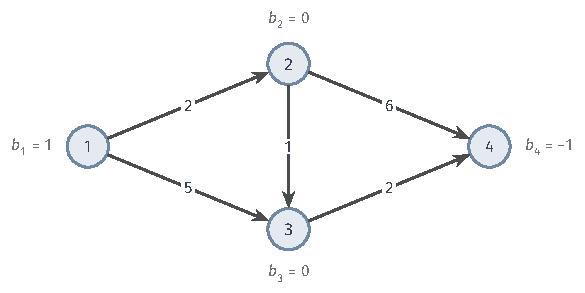
\includegraphics[width=99mm]{figures/05-optimization/01-linear-programming/tikz/lp-network-instance/figure.pdf}
 \caption{一个小网络流实例。弧旁的数字是单位费用$c_{i,j}$，节点旁的$b_i$是净供给：正数表示运出，负数表示收到，零表示只中转。每条弧上的流量$x_{i,j}\geq0$待定。}
 \label{fig:lp-network-instance}
\end{BookInlineFigure}

记弧$(i,j)$上的流量为$x_{i,j}\geq0$。每个节点都要平账：运出的总量减去运入的总量，等于该节点的净供给$b_i$，这称为流量守恒。把五条弧按$(1,2),(1,3),(2,3),(2,4),(3,4)$排列，四个守恒等式合起来就是$\bm{A}\bm{x}=\bm{b}$，其中
\begin{equation}
 \bm{A}=\begin{bmatrix}
 1&1&0&0&0\\
 -1&0&1&1&0\\
 0&-1&-1&0&1\\
 0&0&0&-1&-1
 \end{bmatrix},\qquad
 \bm{b}=\begin{bmatrix}1\\0\\0\\-1\end{bmatrix}.
 \label{eq:lp-network-data}
\end{equation}
$\bm{A}$的每一列对应一条弧，在弧的起点处为$+1$，在终点处为$-1$，其余为零，它是有向图的关联矩阵。

费用向量是$\bm{c}=(2,5,1,6,2)^\top$，总费用$\bm{c}^\top\bm{x}$是线性函数。于是最小费用的运送方案由下面的问题决定：
\[
 \min_{\bm{x}}\ \bm{c}^\top\bm{x}
 \quad\text{s.t.}\quad\bm{A}\bm{x}=\bm{b},\quad\bm{x}\geq\bm{0}.
\]
这里净供给恰好是把一单位货物从节点$1$送到节点$4$，所以问题就是求最短路。若某条弧还有容量上限$x_{i,j}\leq u_{i,j}$，只需多加一条不等式。图上这些问题的专门算法可参考\BookChapterRef{chap:min-cost-flow}{卷三第7章“最小费用流”}，本章只把它们当作线性规划的实例。

\paragraph{标准型}
比较两个模型：资源配置用“$\leq$”约束一般的线性组合，网络流用等式，只把不等号留给单个变量。第二种写法对计算更方便。一组等式可以用线性代数处理，而不等式全部成了“某个坐标非负”，这是最简单的一种不等式。我们把它定为统一的形式。

\begin{definition}[线性规划的标准型]
 \label{def:lp-standard}
 给定$\bm{A}\in\mathbb{R}^{m\times n}$、$\bm{b}\in\mathbb{R}^m$和$\bm{c}\in\mathbb{R}^n$，问题
 \begin{equation}
  \min_{\bm{x}\in\mathbb{R}^n}\ \bm{c}^\top\bm{x}
  \quad\text{s.t.}\quad\bm{A}\bm{x}=\bm{b},\quad\bm{x}\geq\bm{0}
  \label{eq:lp-standard}
 \end{equation}
 称为线性规划的\term{标准型}（standard form），它的可行集记为
 \begin{equation}
  \bm{C}=\{\bm{x}\in\mathbb{R}^n:\bm{A}\bm{x}=\bm{b},\ \bm{x}\geq\bm{0}\}.
  \label{eq:lp-feasible-set}
 \end{equation}
 $\bm{A}$的第$j$列记为$\bm{a}_j=\bm{A}_{:,j}$，最优值记为$p^\star$。
\end{definition}

可以把标准型想成一本账：每个等式是一笔必须平的账，每个变量是一项不能为负的余额。这个比喻只说明约束的形式，并不表示变量都有“余额”的含义。

\paragraph{改写成标准型}
一般的线性规划可以逐项改写。每一步都要说清新旧问题的解怎样相互对应，下面逐种列出。

\emph{最大化改为最小化。}最大化$\bm{p}^\top\bm{x}$与最小化$(-\bm{p})^\top\bm{x}$的最优解相同，最优值互为相反数。

\emph{小于等于约束。}对$\bm{g}^\top\bm{x}\leq h$，引入新变量$s=h-\bm{g}^\top\bm{x}$，约束等价于
\begin{equation}
 \bm{g}^\top\bm{x}+s=h,\qquad s\geq0.
 \label{eq:lp-slack}
\end{equation}
$s$称为\term{松弛变量}（slack variable），它是这条约束还剩的余量。

\emph{大于等于约束。}对$\bm{g}^\top\bm{x}\geq h$，减去\term{剩余变量}（surplus variable）$s=\bm{g}^\top\bm{x}-h\geq0$，得到$\bm{g}^\top\bm{x}-s=h$。

\emph{变量有上下界。}若$x_j\geq l_j$，令$x_j'=x_j-l_j\geq0$；若$x_j\leq u_j$，把它当作一条“小于等于”约束加松弛变量。

\emph{无符号限制的变量。}这样的变量称为\term{自由变量}（free variable）。把它写成两个非负变量之差：
\begin{equation}
 x_j=x_j^{+}-x_j^{-},\qquad x_j^{+}\geq0,\quad x_j^{-}\geq0.
 \label{eq:lp-free-split}
\end{equation}

\begin{example}[车间问题的标准型]
 \label{ex:lp-workshop-standard}
 为工时和原料分别引入松弛变量$x_3,x_4\geq0$，把最大化利润改成最小化利润的相反数，就得到$n=4$，$m=2$的标准型，数据是
 \begin{equation}
  \bm{A}=\begin{bmatrix}1&1&1&0\\2&1&0&1\end{bmatrix},\quad
  \bm{b}=\begin{bmatrix}4\\6\end{bmatrix},\quad
  \bm{c}=\begin{bmatrix}-3\\-2\\0\\0\end{bmatrix}.
  \label{eq:lp-workshop-standard}
 \end{equation}
 第~\ref{chap:optimization}章的解$(x_1,x_2)=(2,2)$对应$\bm{x}=(2,2,0,0)^\top$，工时和原料都恰好用完，目标值是$-10$。
\end{example}

松弛变量的意义可以直接在图上读出。图~\ref{fig:lp-slack-meaning}中，取产量$(1,1)$，代入得到
\[
 x_3=4-1-1=2,\qquad x_4=6-2-1=3.
\]
也就是工时还剩$2$，原料还剩$3$。$x_3=0$恰好是工时约束的边界，$x_3=2$是与边界平行的另一条直线。平面上每个点都对应一组松弛变量的值，点走到哪条边界上，对应的松弛变量就降为零。

\begin{BookInlineFigure}
 \centering
 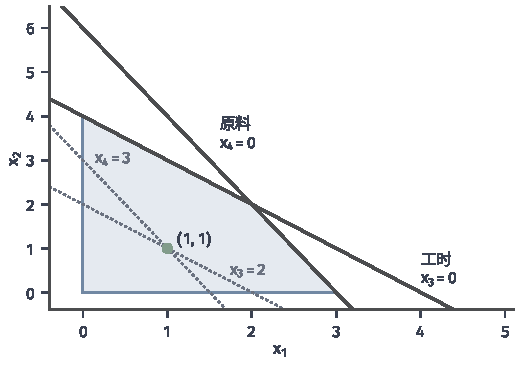
\includegraphics[width=88mm]{figures/05-optimization/01-linear-programming/matplotlib/lp-slack-meaning/figure.pdf}
 \caption{车间问题的松弛变量。深灰粗线是约束取等号的边界，也就是$x_3=0$和$x_4=0$。过绿点$(1,1)$的两条灰色点线是与边界平行的直线，在它们上面$x_3=2$，$x_4=3$，表示这一产量剩下的工时和原料。}
 \label{fig:lp-slack-meaning}
\end{BookInlineFigure}

\paragraph{改写保留了什么}
松弛变量的引入是一一对应的。原问题的可行点$\bm{x}$对应新问题的可行点$(\bm{x},\bm{b}-\bm{A}\bm{x})$，反过来，丢掉松弛变量就回到原来的点。目标值不变，因为松弛变量的费用是零。这个对应是仿射映射，保持线段和中点，所以可行集的形状也保留下来：车间的四边形搬进了$\mathbb{R}^4$，还是同一个四边形。

自由变量的分解不同。从分解后的可行点总能算出原来的$x_j$，目标值相同，所以最优值和最优解的集合不变。但同一个$x_j$有无穷多种写法，图~\ref{fig:lp-free-split}中$(x^{+},x^{-})=(1,0)$和$(3,2)$都表示$x=1$。

\begin{BookInlineFigure}
 \centering
 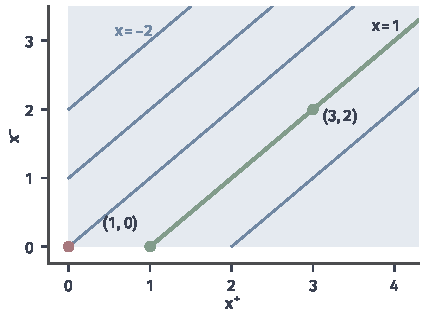
\includegraphics[width=72mm]{figures/05-optimization/01-linear-programming/matplotlib/lp-free-split/figure.pdf}
 \caption{自由变量的分解$x=x^{+}-x^{-}$。浅蓝区域是分解后允许的第一象限，每条斜线上的点代表同一个$x$，绿色粗线是$x=1$。原来的直线变成了一个象限，红点$(0,0)$是这个象限唯一的角点，它在原来的直线上只是普通的一点$x=0$。}
 \label{fig:lp-free-split}
\end{BookInlineFigure}

分解后新问题的最优解可能不唯一，例如沿斜线同时增大$x^{+}$和$x^{-}$，目标值不变。分解还会凭空造出角点：实数轴没有角，第一象限却有角点$(0,0)$。下一节谈顶点时要记住这一点。表~\ref{tab:lp-transformations}汇总了各种改写的效果。

\begin{BookInlineTable}
 \centering
 \begin{tabular}{lll}
  \toprule
  改写 & 解的对应 & 变化 \\
  \midrule
  最大改最小 & 最优解相同 & 最优值变号 \\
  加松弛或剩余变量 & 一一对应 & 变量增加，形状不变 \\
  变量平移 & 一一对应 & 平移可行集 \\
  自由变量分解 & 多对一 & 可能多出角点和最优解 \\
  \bottomrule
 \end{tabular}
 \caption{改写成标准型时各步保留的内容。每一步都保持最优值（或只差符号与常数），并且可以从新问题的解算出原问题的解。}
 \label{tab:lp-transformations}
\end{BookInlineTable}

\paragraph{冗余等式与满行秩}
下一节要从$\bm{A}$中选出可逆的方阵，这需要$\bm{A}$的行没有多余。网络流的矩阵~\eqref{eq:lp-network-data}就有多余的行：每一列恰有一个$+1$和一个$-1$，所以四行相加是零向量，第四行是前三行之和的相反数。$\bm{b}$的分量相加也是零，这说明总供给等于总需求，等式组是相容的。

一般的处理分两步。先检查等式组是否相容，也就是比较$\operatorname{rank}\bm{A}$和增广矩阵的秩：
\[
 \operatorname{rank}\bm{A}=\operatorname{rank}\bigl[\bm{A}\ \ \bm{b}\bigr].
\]
若上式不成立，等式组无解，可行集是空集，问题到此回答完毕。在网络中这对应总供给不等于总需求，货物无处可去。

若相容且$\operatorname{rank}\bm{A}=r<m$，就选出$r$个线性无关的行，其余的行是它们的线性组合，右端也是相应的组合，删去后解集不变。网络的例子里删去第四行即可，剩下三行线性无关，这只要看弧$(1,2),(2,3),(3,4)$三列组成的$3\times3$子矩阵，它是可逆的三角矩阵。秩判别和选主元消元的做法可参考\BookChapterRef{chap:linear-solution-selection}{卷二第11章“线性方程与最小二乘的选解”}。

以后凡涉及基矩阵，都假设已完成这一步，即
\begin{equation}
 \operatorname{rank}\bm{A}=m\leq n.
 \label{eq:lp-full-row-rank}
\end{equation}
车间问题的$\bm{A}$含有单位矩阵，自动满行秩。

\section{基本可行解}
\label{sec:lp-basic-solutions}

线性规划的最优解是否一定落在角点上，角点又怎样用矩阵计算出来？车间问题里这一点靠眼睛看到，变量多了就要靠下面的定义和定理。

\paragraph{多面体与极点}
车间的四边形由四个半平面相交而成。一般地，满足$\bm{g}\neq\bm{0}$的集合$\{\bm{x}:\bm{g}^\top\bm{x}\leq h\}$称为\term{半空间}（halfspace），有限个半空间的交称为\term{多面体}（polyhedron）。写成矩阵形式，就是
\begin{equation}
 \bm{Q}=\{\bm{x}\in\mathbb{R}^n:\bm{G}\bm{x}\leq\bm{h}\},
 \label{eq:lp-polyhedron}
\end{equation}
其中$\bm{G}$的行数有限。等式可以写成两条方向相反的不等式，所以标准型的可行集$\bm{C}$也是多面体。半空间是闭凸集，有限个闭凸集的交仍是闭凸集，多面体因此是闭凸集。

“角点”需要一个不依赖图形的说法。观察图~\ref{fig:lp-extreme-midpoint}：内部的点是某条可行线段的中点，边上的点也是，只不过线段只能沿边摆放。顶点不同，过它的线段无论怎么摆，总有一端跑到可行集外面。

\begin{BookInlineFigure}
 \centering
 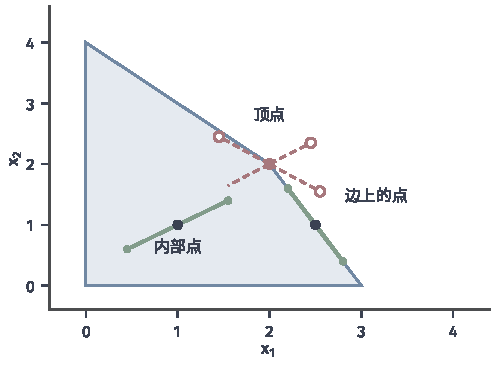
\includegraphics[width=84mm]{figures/05-optimization/01-linear-programming/matplotlib/lp-extreme-midpoint/figure.pdf}
 \caption{三种位置的点。深色的内部点和边上的点都是一条可行线段（绿色）的中点。红点$(2,2)$是顶点，过它的线段（红色虚线）总有一端落在四边形外（空心点），所以它不是任何可行线段的中点。}
 \label{fig:lp-extreme-midpoint}
\end{BookInlineFigure}

\begin{definition}[极点]
 \label{def:lp-extreme-point}
 设$\bm{Q}$是凸集，$\bm{x}\in\bm{Q}$。若$\bm{u},\bm{v}\in\bm{Q}$且$\bm{x}=(\bm{u}+\bm{v})/2$只有在$\bm{u}=\bm{v}=\bm{x}$时才成立，就称$\bm{x}$是$\bm{Q}$的\term{极点}（extreme point）。
\end{definition}

对多面体，极点也称为顶点，本章两种说法通用。

\paragraph{基与基本解}
标准型的可行点要满足$m$个等式，却有$n$个未知数，还剩$n-m$个自由度。平面上的顶点是让两条约束同时取等号得到的，在标准型里，取等号的办法是让坐标变成零。于是自然的做法是：让$n-m$个坐标取零，用$m$个等式解出其余$m$个坐标。

能否解出，取决于留下的那$m$列是否线性无关。

\begin{definition}[基与基本可行解]
 \label{def:lp-basic-solution}
 设$\bm{A}$满行秩。取$m$个下标组成集合$B$，其余下标组成$N$。若由$B$中各列构成的方阵$\bm{A}_B$可逆，就称$B$为一个基，$\bm{A}_B$为\term{基矩阵}（basis matrix）。令
 \begin{equation}
  \bm{x}_B=\bm{A}_B^{-1}\bm{b},\qquad\bm{x}_N=\bm{0},
  \label{eq:lp-basic-solution}
 \end{equation}
 所得的$\bm{x}$称为基$B$对应的\term{基本解}（basic solution），$\bm{x}_B$和$\bm{x}_N$的分量分别称为基分量和非基分量。若还有$\bm{x}_B\geq\bm{0}$，就称$\bm{x}$为\term{基本可行解}（basic feasible solution），$B$为可行基。
\end{definition}

基本解满足全部等式，但不一定非负，所以不一定可行。在车间问题~\eqref{eq:lp-workshop-standard}中，$\bm{A}$的四列任取两列都线性无关，共有$\binom{4}{2}=6$个基。以$B=\{1,4\}$为例，令$x_2=x_3=0$，两个等式变成
\[
 x_1=4,\qquad 2x_1+x_4=6.
\]
解得$x_1=4$，$x_4=-2$。分量为负，这个基本解不可行：产量$(4,0)$用掉的原料比库存多$2$。表~\ref{tab:lp-six-bases}列出了全部六个基本解。

\begin{BookInlineTable}
 \centering
 \begin{tabular}{cccc}
  \toprule
  基$B$ & $\bm{x}=(x_1,x_2,x_3,x_4)$ & 平面上的点 & 是否可行\\
  \midrule
  $\{3,4\}$ & $(0,0,4,6)$ & $(0,0)$ & 可行\\
  $\{1,3\}$ & $(3,0,1,0)$ & $(3,0)$ & 可行\\
  $\{2,4\}$ & $(0,4,0,2)$ & $(0,4)$ & 可行\\
  $\{1,2\}$ & $(2,2,0,0)$ & $(2,2)$ & 可行\\
  $\{1,4\}$ & $(4,0,0,-2)$ & $(4,0)$ & 不可行\\
  $\{2,3\}$ & $(0,6,-2,0)$ & $(0,6)$ & 不可行\\
  \bottomrule
 \end{tabular}
 \caption{车间问题的六个基本解。可行的四个恰好是四边形的四个顶点。}
 \label{tab:lp-six-bases}
\end{BookInlineTable}

图~\ref{fig:lp-basic-solutions}把这六个点画在平面上。它们正是四条边界直线的两两交点：选定基，就是选定哪两个坐标取零，也就是选定哪两条边界同时取等号。

\begin{BookInlineFigure}
 \centering
 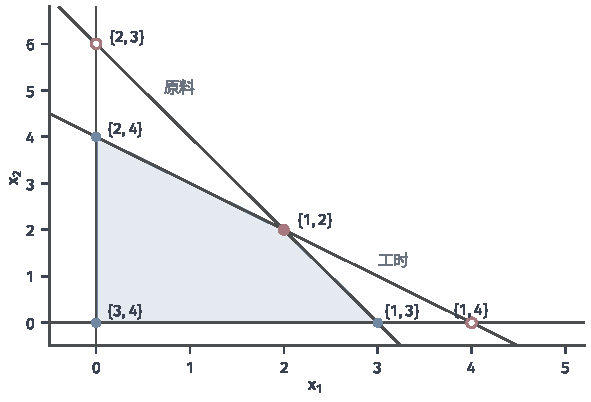
\includegraphics[width=100mm]{figures/05-optimization/01-linear-programming/matplotlib/lp-basic-solutions/figure.pdf}
 \caption{车间问题的六个基本解，点旁标出对应的基。四条直线是$x_1=0$、$x_2=0$和工时、原料两条约束的边界。实心点是四个基本可行解，其中红点$(2,2)$最优；红色空心点$(4,0)$和$(0,6)$的基本解有负分量，落在可行域外。}
 \label{fig:lp-basic-solutions}
\end{BookInlineFigure}

\paragraph{基本可行解就是极点}
表中四个可行的基本解恰好是四个顶点，这不是巧合。下面的定理把代数对象和几何对象连起来，判别的依据是矩阵的秩：只看正分量所在的列。

\begin{theorem}[基本可行解与极点]
 \label{thm:lp-bfs-extreme}
 设$\bm{A}$满行秩，$\bm{x}\in\bm{C}$，$J=\{j:x_j>0\}$。下面三条等价：
 \begin{enumerate}
  \item $\bm{x}$是$\bm{C}$的极点；
  \item 列$\{\bm{a}_j:j\in J\}$线性无关；
  \item $\bm{x}$是某个基对应的基本可行解。
 \end{enumerate}
\end{theorem}

\begin{proof}
 先证(1)推出(2)。假设这些列线性相关，则有不全为零的系数$w_j$（$j\in J$）使$\sum_{j\in J}w_j\bm{a}_j=\bm{0}$。把$\bm{w}$在$J$以外的分量补成零，就有
 \[
  \bm{A}\bm{w}=\bm{0},\qquad\bm{w}\neq\bm{0}.
 \]
 $J$上的$x_j$都是正数，取足够小的$\varepsilon>0$，可使$\bm{x}\pm\varepsilon\bm{w}\geq\bm{0}$。再由$\bm{A}\bm{w}=\bm{0}$知这两个点都满足等式，都可行。它们不相等，而$\bm{x}$是它们的中点，与$\bm{x}$是极点矛盾。

 再证(2)推出(3)。线性无关的列不超过$m$个，所以$\lvert J\rvert\leq m$。$\bm{A}$满行秩，它的列张成$\mathbb{R}^m$，可以再补入若干列，把$\{\bm{a}_j:j\in J\}$扩充成$\mathbb{R}^m$的一组基，相应的下标集记为$B\supseteq J$。于是$\bm{A}_B$可逆，$B$之外的分量都不在$J$中，所以$\bm{x}_N=\bm{0}$。代入等式得到
 \[
  \bm{A}_B\bm{x}_B=\bm{b},\qquad\text{即}\qquad\bm{x}_B=\bm{A}_B^{-1}\bm{b}.
 \]
 又$\bm{x}$可行，故$\bm{x}_B\geq\bm{0}$，它是基$B$的基本可行解。

 最后证(3)推出(1)。设$\bm{x}$是基$B$的基本可行解，且$\bm{x}=(\bm{u}+\bm{v})/2$，$\bm{u},\bm{v}\in\bm{C}$。对$j\in N$，有$u_j+v_j=2x_j=0$，又$u_j,v_j\geq0$，所以$u_j=v_j=0$。于是$\bm{A}_B\bm{u}_B=\bm{b}$，由$\bm{A}_B$可逆得到
 \[
  \bm{u}_B=\bm{A}_B^{-1}\bm{b}=\bm{x}_B.
 \]
 所以$\bm{u}=\bm{x}$，同理$\bm{v}=\bm{x}$。
\end{proof}

定理中的秩条件有直接的几何解释。在点$\bm{x}$处取等号的约束是$m$个等式和$n-\lvert J\rvert$个“坐标为零”。把它们的系数排成矩阵$\bm{M}$，$\bm{M}\bm{v}=\bm{0}$说的是
\[
 \bm{v}_{J^c}=\bm{0},\qquad\bm{A}_J\bm{v}_J=\bm{0}.
\]
其中$J^c$是$J$的补集。所以$\bm{M}$的列满秩，也就是取等号的约束能唯一确定一个点，当且仅当$\bm{A}_J$的列线性无关。“$n$个线性无关的约束取等号”和“基矩阵可逆”是同一件事的两种说法。

用车间问题验证一下。点$(5/2,1)$对应$\bm{x}=(5/2,1,1/2,0)^\top$，正分量在第$1,2,3$列，三列放在$\mathbb{R}^2$中线性相关，取
\[
 \bm{w}=(-1,2,-1,0)^\top,\qquad\bm{A}\bm{w}=\bm{0}.
\]
$\bm{x}\pm\varepsilon\bm{w}$都可行，所以它不是极点，在图上它是原料边界中间的一点。点$(2,2)$对应$\bm{x}=(2,2,0,0)^\top$，第$1,2$列线性无关，它是极点。

基的个数不超过$\binom{n}{m}$，所以极点只有有限个。最优解若能在极点取得，问题就从无穷多个候选变成了有限多个。

\paragraph{最优解可以在基本可行解中取得}
下面证明这确实成立。证明的想法很具体：任取一个可行点，如果它的正分量对应的列线性相关，就有一个方向可以沿着走，目标不变差，直到某个正分量降到零。正分量越来越少，最后得到一个基本可行解。

\begin{lemma}[推向基本可行解]
 \label{lem:lp-push}
 设$\bm{A}$满行秩，且$\bm{c}^\top\bm{x}$在$\bm{C}$上有下界。则对每个$\bm{x}\in\bm{C}$，存在基本可行解$\widehat{\bm{x}}$，使
 \begin{equation}
  \bm{c}^\top\widehat{\bm{x}}\leq\bm{c}^\top\bm{x}.
  \label{eq:lp-push}
 \end{equation}
\end{lemma}

\begin{proof}
 对正分量的个数$\lvert J\rvert$归纳。若列$\{\bm{a}_j:j\in J\}$线性无关，由定理~\ref{thm:lp-bfs-extreme}，$\bm{x}$本身就是基本可行解。

 否则取$\bm{w}\neq\bm{0}$，满足$\bm{A}\bm{w}=\bm{0}$，且$w_j=0$对$j\notin J$成立。必要时用$-\bm{w}$代替$\bm{w}$，可使$\bm{c}^\top\bm{w}\leq0$。先说明可以假设$\bm{w}$有负分量。

 若$\bm{w}\geq\bm{0}$且$\bm{c}^\top\bm{w}<0$，则对一切$t\geq0$，点$\bm{x}+t\bm{w}$可行，目标值$\bm{c}^\top\bm{x}+t\bm{c}^\top\bm{w}$趋于$-\infty$，与有下界矛盾，这种情形不出现。若$\bm{w}\geq\bm{0}$且$\bm{c}^\top\bm{w}=0$，就把$\bm{w}$换成$-\bm{w}$，此时$\bm{c}^\top\bm{w}$仍为零，而$\bm{w}$有了负分量。

 现在令
 \[
  t^\star=\min_{j:\,w_j<0}\frac{x_j}{-w_j},\qquad\bm{x}'=\bm{x}+t^\star\bm{w}.
 \]
 负分量只出现在$J$中，那里$x_j>0$，所以$t^\star>0$。$t^\star$的取法保证$\bm{x}'\geq\bm{0}$，又$\bm{A}\bm{x}'=\bm{b}$，所以$\bm{x}'$可行，并且
 \[
  \bm{c}^\top\bm{x}'=\bm{c}^\top\bm{x}+t^\star\bm{c}^\top\bm{w}\leq\bm{c}^\top\bm{x}.
 \]

 $J$之外的分量保持为零，取到最小值的分量变成零，所以$\bm{x}'$的正分量个数严格减少。对$\bm{x}'$用归纳假设，即得$\widehat{\bm{x}}$。
\end{proof}

用车间问题走一遍。从可行点$(x_1,x_2)=(1,1)$出发，四个坐标是$\bm{x}=(1,1,2,3)^\top$，目标值$-5$。四列放在$\mathbb{R}^2$中必然线性相关，可以取下面的方向，并算出步长：
\[
 \bm{w}=(1,0,-1,-2)^\top,\qquad\bm{c}^\top\bm{w}=-3,\qquad
 t^\star=\min\Bigl\{\frac{2}{1},\frac{3}{2}\Bigr\}=\frac32.
\]
走完得到第一个新点，$x_4$降到了零：
\[
 \bm{x}'=\Bigl(\frac52,1,\frac12,0\Bigr)^\top,\qquad\bm{c}^\top\bm{x}'=-\frac{19}{2}.
\]

此时还剩三个正分量，第$1,2,3$列在$\mathbb{R}^2$中仍然线性相关。满足$w_4=0$的零空间方向是$(1,-2,1,0)^\top$，它的目标变化率是$+1$，所以取反方向，并求步长：
\[
 \bm{w}=(-1,2,-1,0)^\top,\qquad\bm{c}^\top\bm{w}=-1,\qquad
 t^\star=\min\Bigl\{\frac{5/2}{1},\frac{1/2}{1}\Bigr\}=\frac12.
\]
走完得到
\[
 \bm{x}''=(2,2,0,0)^\top,\qquad\bm{c}^\top\bm{x}''=-10.
\]
正分量只剩两个，对应的列线性无关，这就是基本可行解。图~\ref{fig:lp-push-to-vertex}显示了这两步：先水平走到原料边界，再沿边界走到顶点。这里碰巧到达了最优解，一般只能保证目标不变差。

\begin{BookInlineFigure}
 \centering
 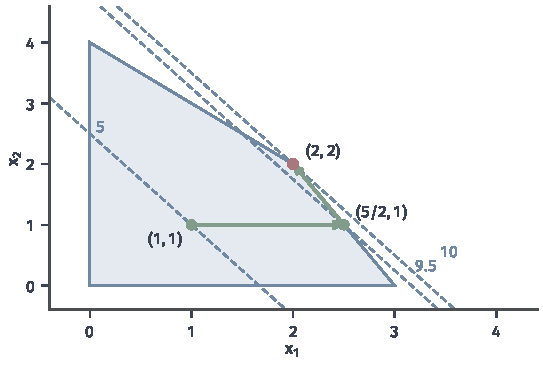
\includegraphics[width=92mm]{figures/05-optimization/01-linear-programming/matplotlib/lp-push-to-vertex/figure.pdf}
 \caption{引理~\ref{lem:lp-push}在车间问题上的两步。绿色箭头从$(1,1)$（四个正分量）走到$(5/2,1)$（三个正分量），再走到顶点$(2,2)$（两个正分量）。蓝色虚线是利润等于$5$、$9.5$、$10$的等值线，每一步都不使利润变小。}
 \label{fig:lp-push-to-vertex}
\end{BookInlineFigure}

\begin{theorem}[最优基本可行解的存在]
 \label{thm:lp-optimal-bfs}
 设$\bm{A}$满行秩。若标准型~\eqref{eq:lp-standard}可行且最优值有限，则最优值能够取到，并且至少有一个最优解是基本可行解。特别地，非空的$\bm{C}$至少有一个极点。
\end{theorem}

\begin{proof}
 基本可行解至多有$\binom{n}{m}$个，由引理~\ref{lem:lp-push}（对$\bm{C}$中任一点使用），它们至少有一个。在这有限个点中取目标值最小的$\bm{x}^\star$。对任意$\bm{x}\in\bm{C}$，引理给出基本可行解$\widehat{\bm{x}}$，于是
 \[
  \bm{c}^\top\bm{x}\geq\bm{c}^\top\widehat{\bm{x}}\geq\bm{c}^\top\bm{x}^\star.
 \]
 所以$\bm{x}^\star$是最优解。最后一句取$\bm{c}=\bm{0}$即得。
\end{proof}

定理中“$\bm{A}$满行秩”只是为了让基有定义，这一点上一节已经保证。这个结论比一般的存在定理强。第~\ref{chap:optimization}章的$e^x$有下界却取不到下确界，而标准型线性规划只要最优值有限，就一定取得到，并不要求可行集有界。条件里的“可行”和“最优值有限”各自排除一种结局，图~\ref{fig:lp-three-outcomes}画出了线性规划的三种情形。

\begin{BookInlineFigure}
 \centering
 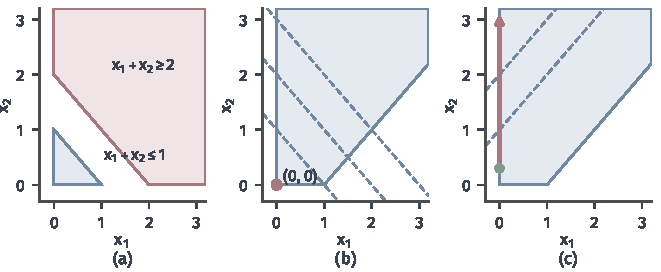
\includegraphics[width=112mm]{figures/05-optimization/01-linear-programming/matplotlib/lp-three-outcomes/figure.pdf}
 \caption{线性规划的三种结局。(a)~第一象限中两条约束围成的区域不相交，问题不可行。(b)~可行域$\{\bm{x}\geq\bm{0},\ x_1-x_2\leq1\}$无界，但最小化$x_1+x_2$（蓝色虚线是等值线）的最优解存在，是红点$(0,0)$。(c)~同一可行域上最小化$x_1-x_2$，从绿点沿红色射线一直走，目标趋于$-\infty$，问题无下界。}
 \label{fig:lp-three-outcomes}
\end{BookInlineFigure}

定理只说有一个最优解是基本可行解，不说所有最优解都是。把车间的目标改成最大化$2x_1+x_2$，等值线与原料边界平行，图~\ref{fig:lp-optimal-face}(b)中$(2,2)$和$(3,0)$都最优，它们连线上的每一点也都最优。中点$(5/2,1)$对应$\bm{x}=(5/2,1,1/2,0)^\top$，有三个正分量，多于$m=2$，所以不是基本可行解，却同样最优。

\begin{BookInlineFigure}
 \centering
 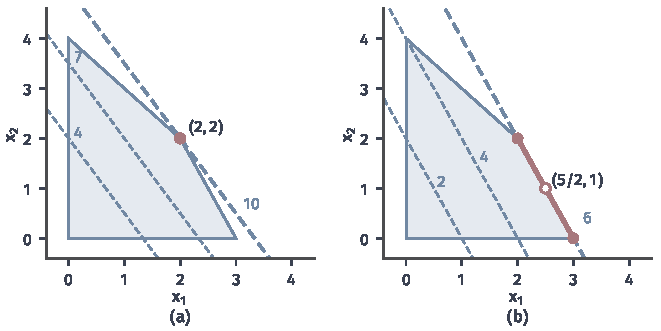
\includegraphics[width=112mm]{figures/05-optimization/01-linear-programming/matplotlib/lp-optimal-face/figure.pdf}
 \caption{等值线平移到最后接触可行域的情形。(a)~最大化$3x_1+2x_2$，粗虚线（利润$10$）只接触顶点$(2,2)$，最优解唯一。(b)~最大化$2x_1+x_2$，粗虚线（值为$6$）与一条边重合，红色线段上都是最优解，其中空心点$(5/2,1)$不是顶点。}
 \label{fig:lp-optimal-face}
\end{BookInlineFigure}

定理把问题化成了有限比较，但枚举全部的基并不现实。$n=100$，$m=50$时，$\binom{n}{m}$约为$1.0\times10^{29}$。需要的是一种不逐个检查、只在相邻顶点之间移动的办法，下面先说清“相邻”是什么意思。

\paragraph{沿边到相邻顶点}
在车间的四边形上，相邻顶点由一条边相连。用基来说，相邻的两个基只差一个下标。设$B$是可行基，$\bar{\bm{x}}$是它的基本可行解，取一个不在$B$中的下标$q$。让$x_q$从零增大，其余非基分量保持为零，基分量必须随之调整，以维持等式。由$\bm{A}_B\bm{x}_B+\bm{a}_qx_q=\bm{b}$解出
\begin{equation}
 \bm{x}_B=\bar{\bm{x}}_B-x_q\bm{u},\qquad\bm{u}=\bm{A}_B^{-1}\bm{a}_q.
 \label{eq:lp-edge-direction}
\end{equation}
这相当于让点沿方向$\bm{d}$移动，其中$d_q=1$，$\bm{d}_B=-\bm{u}$，其余分量为零，并且$\bm{A}\bm{d}=\bm{0}$。

\begin{theorem}[沿边的移动]
 \label{thm:lp-edge-move}
 设$\bm{A}$满行秩，$B$是可行基，$\bar{\bm{x}}$是其基本可行解，$q\notin B$，$\bm{u}$和$\bm{d}$如上。则满足“$x_j=0$对$j\notin B\cup\{q\}$成立”的可行点恰好是$\bar{\bm{x}}+\alpha\bm{d}$，其中$\alpha\geq0$且$\bar{\bm{x}}_B-\alpha\bm{u}\geq\bm{0}$。进一步：
 \begin{enumerate}
  \item 若$\bm{u}$有正分量，且$\bar{\bm{x}}_B>\bm{0}$，记$r$是下式取到最小值的位置，$B(i)$是基中第$i$个下标：
  \begin{equation}
   \alpha^\star=\min_{i:\,u_i>0}\frac{\bar{x}_{B(i)}}{u_i}>0.
   \label{eq:lp-edge-step}
  \end{equation}
  把$B$中的$B(r)$换成$q$得到新基，$\bar{\bm{x}}+\alpha^\star\bm{d}$是新基的基本可行解，且与$\bar{\bm{x}}$不同。
  \item 若$\bm{u}\leq\bm{0}$，则对一切$\alpha\geq0$，$\bar{\bm{x}}+\alpha\bm{d}$都可行。
 \end{enumerate}
\end{theorem}

\begin{proof}
 由式~\eqref{eq:lp-edge-direction}，满足等式且$x_j=0$（$j\notin B\cup\{q\}$）的点完全由$x_q$确定，就是$\bar{\bm{x}}+x_q\bm{d}$。再加上非负条件，得到第一句。

 对情形1，$\bar{\bm{x}}_B>\bm{0}$保证$\alpha^\star>0$，点因此确实移动了。$\alpha^\star$的取法使基分量保持非负，而位置$r$上的分量降为零。新基矩阵可逆：由$\bm{A}_B\bm{u}=\bm{a}_q$，有$\bm{a}_q=\sum_iu_i\bm{a}_{B(i)}$，其中$\bm{a}_{B(r)}$的系数$u_r\neq0$，所以用$\bm{a}_q$替换$\bm{a}_{B(r)}$后列仍线性无关。新点在新基之外的分量都是零，它就是新基的基本可行解。

 对情形2，$\bm{u}\leq\bm{0}$时基分量不减，$\alpha\geq0$都满足非负条件。
\end{proof}

定理的第一句就是“边”的代数含义：$m$个等式和$n-m-1$个坐标为零，共$n-1$个线性无关的条件，只留下一个自由度，可行点构成一条线段或射线。把一个下标换入、另一个换出，这个操作称为换基，它的几何含义在基分量都为正时正是沿边走到相邻顶点。选哪个$q$能改善目标，是第~\ref{chap:simplex-method}章的问题，这里只看移动本身。

在车间问题上从$B=\{3,4\}$，即点$(0,0)$出发，让$x_1$增大。此时$\bm{A}_B=\bm{I}$，于是
\[
 \bm{u}=\bm{a}_1=\begin{bmatrix}1\\2\end{bmatrix},\qquad
 \bar{\bm{x}}_B=\begin{bmatrix}4\\6\end{bmatrix},\qquad
 \alpha^\star=\min\Bigl\{\frac41,\frac62\Bigr\}=3.
\]
最小值由原料的松弛变量$x_4$取到，所以$x_4$换出，点沿下边走到$(3,0)$，新基是$\{1,3\}$，其中基分量$x_1=3$，$x_3=4-3=1$。

再让$x_2$增大。新基矩阵的列是$\bm{a}_1,\bm{a}_3$，解$\bm{A}_B\bm{u}=\bm{a}_2$，并按位置比较：
\[
 \bm{u}=\begin{bmatrix}1/2\\1/2\end{bmatrix},\qquad
 \bar{\bm{x}}_B=\begin{bmatrix}3\\1\end{bmatrix},\qquad
 \alpha^\star=\min\Bigl\{\frac{3}{1/2},\frac{1}{1/2}\Bigr\}=2.
\]
$x_3$先降到零，$x_1$变成$3-2\cdot\frac12=2$，$x_2$变成$2$，点走到$(2,2)$，基变成$\{1,2\}$。图~\ref{fig:lp-pivot-edge}显示了这两次移动和第一次移动中基分量的变化。基$\{3,4\}$和$\{1,2\}$差两个下标，它们的顶点$(0,0)$与$(2,2)$不相邻，连接它们的线段穿过四边形内部，不是边。

\begin{BookInlineFigure}
 \centering
 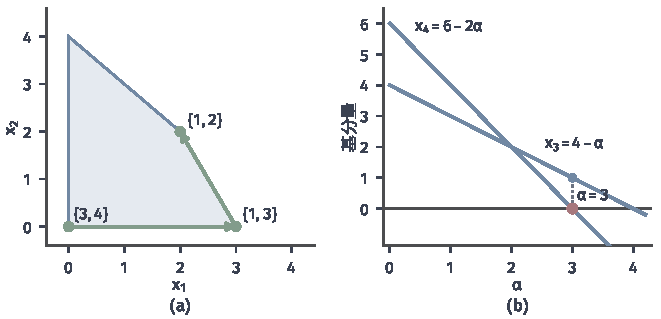
\includegraphics[width=112mm]{figures/05-optimization/01-linear-programming/matplotlib/lp-pivot-edge/figure.pdf}
 \caption{两次换基。(a)~绿色箭头沿边从$(0,0)$到$(3,0)$，再到$(2,2)$，点旁是当时的基。(b)~第一次移动时两个基分量随步长$\alpha$下降，$x_4$在$\alpha=3$处最先到零（红点），此时$x_3=1$。}
 \label{fig:lp-pivot-edge}
\end{BookInlineFigure}

\paragraph{含直线的多面体没有极点}
以上结论都是对标准型说的。它们能推广到什么范围？在平面上考虑带形
\[
 \{(x_1,x_2):0\leq x_2\leq1\}.
\]
最小化$x_2$，最优值$0$在整条直线$x_2=0$上取得，但这个集合没有角点。图~\ref{fig:lp-no-vertex-strip}(a)中，每个点都是左右两个可行点的中点。可见“有最优解就有最优顶点”不是所有多面体都有的性质，缺的是下面的秩条件。

\begin{BookInlineFigure}
 \centering
 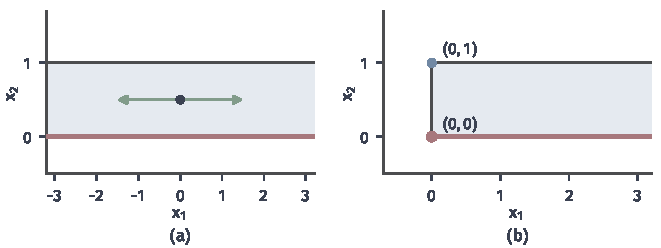
\includegraphics[width=112mm]{figures/05-optimization/01-linear-programming/matplotlib/lp-no-vertex-strip/figure.pdf}
 \caption{极点的存在依赖可行集的形状，目标取$x_2$，红色粗线是最优解集合。(a)~带形含有水平直线，绿色线段说明任一点都是两个可行点的中点，所以没有极点，最优解集合也没有端点。(b)~加上$x_1\geq0$后不再含直线，出现顶点$(0,0)$和$(0,1)$，最优值在顶点$(0,0)$取得。}
 \label{fig:lp-no-vertex-strip}
\end{BookInlineFigure}

\begin{lemma}[多面体的极点]
 \label{lem:lp-polyhedron-vertices}
 设$\bm{Q}=\{\bm{x}:\bm{G}\bm{x}\leq\bm{h}\}$非空，其中$\bm{G}$有$n$列。对$\bm{x}\in\bm{Q}$，记$I(\bm{x})$为取等号的行的下标集。则$\bm{x}$是极点，当且仅当$\bm{G}_{I(\bm{x}),:}$的秩为$n$。进一步，下面三条等价：$\bm{Q}$有极点；$\operatorname{rank}\bm{G}=n$；$\bm{Q}$不含直线。
\end{lemma}

\begin{proof}
 先证第一句。若取等号的行的秩小于$n$，存在$\bm{d}\neq\bm{0}$使这些行与$\bm{d}$的内积都为零。其余的行留有余量，$\varepsilon>0$足够小时$\bm{x}\pm\varepsilon\bm{d}\in\bm{Q}$，所以$\bm{x}$不是极点。反之设秩为$n$，且$\bm{x}=(\bm{u}+\bm{v})/2$，$\bm{u},\bm{v}\in\bm{Q}$。对每个$i\in I(\bm{x})$，两个不超过$h_i$的数平均后等于$h_i$，只能都等于$h_i$，所以$\bm{u}$和$\bm{v}$满足相同的取等号方程组。这个方程组的解唯一，故$\bm{u}=\bm{v}=\bm{x}$。

 再证三条等价。若$\operatorname{rank}\bm{G}<n$，取$\bm{d}\neq\bm{0}$使$\bm{G}\bm{d}=\bm{0}$，则过任一点沿$\bm{d}$的直线都在$\bm{Q}$中，这时由第一句也没有极点。反之若$\bm{Q}$含直线$\bm{x}+t\bm{d}$，则对全部$t\in\mathbb{R}$有$\bm{G}(\bm{x}+t\bm{d})\leq\bm{h}$，只能$\bm{G}\bm{d}=\bm{0}$，秩小于$n$。若有极点，由第一句$\bm{G}$的秩为$n$。

 剩下要证$\operatorname{rank}\bm{G}=n$时有极点。取$\bm{Q}$中使$\operatorname{rank}\bm{G}_{I(\bm{x}),:}$最大的点$\bm{x}$。假设这个秩小于$n$，取$\bm{d}\neq\bm{0}$与取等号的行都正交。由$\operatorname{rank}\bm{G}=n$，$\bm{G}\bm{d}\neq\bm{0}$，必要时换成$-\bm{d}$，可设有一行的内积为正。沿$\bm{d}$走到第一条新约束取等号为止，原来取等号的行仍取等号，新行与$\bm{d}$不正交，不在原来那些行的张成中，秩增大，矛盾。所以这个秩等于$n$，$\bm{x}$是极点。
\end{proof}

标准型中$\bm{G}$含有$-\bm{I}$这一块，秩一定是$n$，所以非负约束自动排除了直线。定理~\ref{thm:lp-optimal-bfs}成立的前提正是这一点。

上一节说自由变量分解会造出角点，这里可以看得很清楚。把带形写成标准型：令$x_1=x_1^{+}-x_1^{-}$，加松弛变量$w$，约束只剩一个等式$x_2+w=1$。基只能是$\{x_2\}$或$\{w\}$，基$\{w\}$给出的基本可行解$(x_1^{+},x_1^{-},x_2,w)=(0,0,0,1)$是最优的。它对应带形中的点$(0,0)$，这个点是最优解，却不是带形的顶点。所以应用定理时要分清：顶点是标准型的顶点，回到原问题后只保证是一个最优解。

\paragraph{退化基与无界可行方向}
基和点的对应还有两种偏差，表现相似，含义却不同，都发生在换基的时候。

第一种是几个基对应同一个点。给车间问题再加一条约束$x_1\leq3$，引入松弛变量$x_5$，得到$m=3$，$n=5$的标准型。可行域没有变化，但顶点$(3,0)$现在有三条边界经过，如图~\ref{fig:lp-degenerate-vertex}。这个点是
\[
 \bm{x}=(3,0,1,0,0)^\top,
\]
只有$x_1,x_3$两个正分量，而基需要三个下标。

\begin{BookInlineFigure}
 \centering
 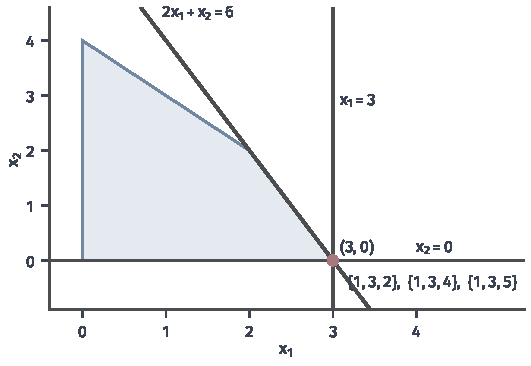
\includegraphics[width=90mm]{figures/05-optimization/01-linear-programming/matplotlib/lp-degenerate-vertex/figure.pdf}
 \caption{退化顶点。加入约束$x_1\leq3$后，四边形没有变，但三条深灰粗线同时经过红点$(3,0)$。第三个基下标取$2$、$4$或$5$，三个基$\{1,3,2\}$、$\{1,3,4\}$、$\{1,3,5\}$都给出这同一个点。}
 \label{fig:lp-degenerate-vertex}
\end{BookInlineFigure}

第三个下标可以取$2$、$4$或$5$，三个基矩阵都可逆，所以三个基给出同一个点，每个基中都有一个取零的基分量。这样的基称为\term{退化基}（degenerate basis），对应的基本可行解称为退化的。此时定理~\ref{thm:lp-edge-move}的条件$\bar{\bm{x}}_B>\bm{0}$不成立。

从基$\{1,3,2\}$（基分量依次为$3,1,0$）出发，让$x_4$增大，解$\bm{A}_B\bm{u}=\bm{a}_4$得到
\[
 \bm{u}=(0,-1,1)^\top,\qquad\alpha^\star=\frac{0}{1}=0.
\]
基变成$\{1,3,4\}$，点却一动不动。“换基”和“走到另一个顶点”在退化时不再是一回事。

第二种是沿某条边可以走到无穷远。取可行域$x_1-x_2\leq1$，$\bm{x}\geq\bm{0}$，写成标准型$x_1-x_2+x_3=1$，这里$m=1$。在基$\{3\}$处，点是$(0,0,1)^\top$。让$x_2$增大：
\[
 u=\bm{A}_B^{-1}\bm{a}_2=-1\leq0.
\]
由定理~\ref{thm:lp-edge-move}的情形2，沿$\bm{d}=(0,1,1)^\top$可以一直走。满足下面条件的$\bm{d}$称为\term{无界可行方向}（unbounded feasible direction）：
\begin{equation}
 \bm{A}\bm{d}=\bm{0},\qquad\bm{d}\geq\bm{0},\qquad\bm{d}\neq\bm{0}.
 \label{eq:lp-recession}
\end{equation}
任何可行点沿它走都不会离开$\bm{C}$。这是可行集形状的性质，与目标无关：可行集无界不等于问题无下界，只有$\bm{c}^\top\bm{d}<0$时目标才沿它趋于$-\infty$。图~\ref{fig:lp-three-outcomes}的(b)与(c)用的正是同一个可行域。表~\ref{tab:lp-degenerate-vs-ray}对比了这两种现象。

\begin{BookInlineTable}
 \centering
 \begin{tabular}{lll}
  \toprule
  & 退化基 & 无界可行方向 \\
  \midrule
  代数表现 & 基分量取零 & $\bm{u}\leq\bm{0}$ \\
  步长 & 可能$\alpha^\star=0$ & 没有上限 \\
  几何含义 & 多余约束过同一顶点 & 可行集沿射线无界 \\
  对目标的影响 & 换基后点和目标值不变 & $\bm{c}^\top\bm{d}<0$时无下界 \\
  \bottomrule
 \end{tabular}
 \caption{退化基与无界可行方向的对比。}
 \label{tab:lp-degenerate-vs-ray}
\end{BookInlineTable}

\section{线性规划的对偶}
\label{sec:lp-duality}

有人告诉我们，车间问题的最优解是$(2,2)$，最大利润是$10$。检查可行性只需代入约束，难的是确认没有更好的产量。怎样给出一份不依赖求解过程、能当场核对的最优性证据？答案来自第~\ref{chap:optimization}章用过的办法，把约束加起来，只是这次要系统地做。

\paragraph{给约束配权重}
把工时约束乘以$u_1\geq0$，原料约束乘以$u_2\geq0$，再相加。权重非负，不等号方向不变，得到
\[
 (u_1+2u_2)x_1+(u_1+u_2)x_2\leq4u_1+6u_2.
\]
如果左边的系数“盖得住”利润系数，也就是
\[
 u_1+2u_2\geq3,\qquad u_1+u_2\geq2,
\]
那么由$x_1,x_2\geq0$，任何可行产量的利润都不超过$4u_1+6u_2$。

不同的权重给出不同的上界。下面四组权重都满足上述条件：
\[
 \bm{u}=(2,1)\to14,\quad(3,0)\to12,\quad(0,2)\to12,\quad(1,1)\to10.
\]
最后一个上界$10$恰好等于$(2,2)$的利润，所以$(2,2)$最优。这一行计算不依赖任何算法，谁都可以复核。

权重可以读成资源的价格。设想有人想买下车间全部的工时和原料，出价$u_1,u_2$。车间只在卖资源不比自己生产亏时才肯卖，这就是上面的两个不等式。买方希望总价$4u_1+6u_2$尽量低，寻找最低总价就是寻找最紧的上界，于是有问题
\begin{equation}
 \min_{u_1,u_2}\ 4u_1+6u_2
 \quad\text{s.t.}\quad u_1+2u_2\geq3,\quad u_1+u_2\geq2,\quad u_1,u_2\geq0.
 \label{eq:lp-workshop-prices}
\end{equation}
图~\ref{fig:lp-dual-bounds}(a)是这个问题的可行域，最低总价$10$在$(1,1)$取得。图~\ref{fig:lp-dual-bounds}(b)把两边的数放在同一条数轴上：每个产量的利润都在每个价格的总价左边，两者在$10$处相遇。这正是“上下界夹逼”。买卖的故事只用来说明不等式的方向，并不表示真有这样一个市场，价格只是一组使不等式成立的数。

\begin{BookInlineFigure}
 \centering
 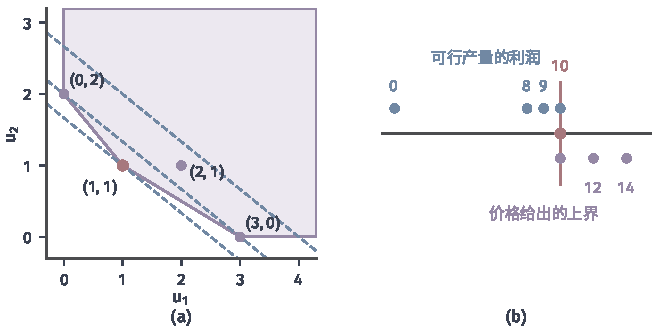
\includegraphics[width=112mm]{figures/05-optimization/01-linear-programming/matplotlib/lp-dual-bounds/figure.pdf}
 \caption{资源价格给出的上界。(a)~浅紫区域是满足式~\eqref{eq:lp-workshop-prices}约束的价格$(u_1,u_2)$，蓝色虚线是总价$10,12,16$的等值线，红点$(1,1)$是最低总价。(b)~数轴上方的蓝点是四个顶点的利润$0,8,9,10$，下方的紫点是四组价格的总价$10,12,14$，红线标出两侧在$10$处相遇。}
 \label{fig:lp-dual-bounds}
\end{BookInlineFigure}

\paragraph{标准型的对偶问题}
对标准型~\eqref{eq:lp-standard}做同样的事。约束是等式，乘以任意实数都不改变等号，所以第$i$个等式的权重$y_i$没有符号限制。把等式按权重相加，得到
\[
 \bm{y}^\top\bm{A}\bm{x}=\bm{b}^\top\bm{y}.
\]
我们想用左边给目标$\bm{c}^\top\bm{x}$找下界。记两者系数的差为$\bm{s}=\bm{c}-\bm{A}^\top\bm{y}$，则
\[
 \bm{c}^\top\bm{x}=\bm{y}^\top\bm{A}\bm{x}+\bm{s}^\top\bm{x}=\bm{b}^\top\bm{y}+\bm{s}^\top\bm{x}.
\]
只要$\bm{s}\geq\bm{0}$，由$\bm{x}\geq\bm{0}$知$\bm{s}^\top\bm{x}\geq0$，于是$\bm{b}^\top\bm{y}$就是下界。求最好的下界，就得到下面的问题。

\begin{definition}[线性规划的对偶问题]
 \label{def:lp-dual}
 标准型~\eqref{eq:lp-standard}的\term{对偶问题}（dual problem）是
 \begin{equation}
  \max_{\bm{y}\in\mathbb{R}^m,\ \bm{s}\in\mathbb{R}^n}\ \bm{b}^\top\bm{y}
  \quad\text{s.t.}\quad\bm{A}^\top\bm{y}+\bm{s}=\bm{c},\quad\bm{s}\geq\bm{0},
  \label{eq:lp-dual}
 \end{equation}
 其中$\bm{y}$没有符号限制，$\bm{s}$称为\term{对偶松弛}（dual slack），最优值记为$d^\star$。相对地，式~\eqref{eq:lp-standard}称为\term{原始问题}（primal problem）。
\end{definition}

对偶的每个$s_j$对应原始的一个变量$x_j$，对偶的每个$y_i$对应原始的一个等式。把车间问题的标准型~\eqref{eq:lp-workshop-standard}代入，得到
\[
 s_1=-3-y_1-2y_2,\quad s_2=-2-y_1-y_2,\quad s_3=-y_1,\quad s_4=-y_2.
\]
$s_3,s_4\geq0$说的是$y_1,y_2\leq0$，这个符号来自松弛变量的列。令$\bm{u}=-\bm{y}$，$s_1,s_2\geq0$就是式~\eqref{eq:lp-workshop-prices}的两个不等式，对偶目标$4y_1+6y_2$变为$-(4u_1+6u_2)$。两种写法只差一个符号，因为这里把最大利润改成了最小化相反数。

\begin{theorem}[弱对偶]
 \label{thm:lp-weak-duality}
 若$\bm{x}$对原始问题可行，$(\bm{y},\bm{s})$对对偶问题可行，则
 \begin{equation}
  \bm{c}^\top\bm{x}-\bm{b}^\top\bm{y}=\bm{x}^\top\bm{s}\geq0.
  \label{eq:lp-weak-duality}
 \end{equation}
 特别地$d^\star\leq p^\star$；若$\bm{x}^\top\bm{s}=0$，则$\bm{x}$和$(\bm{y},\bm{s})$分别是两个问题的最优解。
\end{theorem}

\begin{proof}
 把$\bm{c}=\bm{A}^\top\bm{y}+\bm{s}$代入，再用$\bm{A}\bm{x}=\bm{b}$，得到
 \[
  \bm{c}^\top\bm{x}=\bm{y}^\top\bm{A}\bm{x}+\bm{s}^\top\bm{x}=\bm{b}^\top\bm{y}+\bm{x}^\top\bm{s}.
 \]
 两个向量都非负，所以$\bm{x}^\top\bm{s}\geq0$。

 若$\bm{x}^\top\bm{s}=0$，则$\bm{c}^\top\bm{x}=\bm{b}^\top\bm{y}$。任何其他原始可行点的目标值都不小于$\bm{b}^\top\bm{y}$，任何其他对偶可行点的目标值都不大于$\bm{c}^\top\bm{x}$，所以两者都最优。
\end{proof}

这个结论称为\term{弱对偶}（weak duality）。差$\bm{c}^\top\bm{x}-\bm{b}^\top\bm{y}$称为这对可行点的\term{对偶间隙}（duality gap）。它同时控制了两边：$\bm{c}^\top\bm{x}-p^\star$不超过间隙，$d^\star-\bm{b}^\top\bm{y}$也不超过间隙。

条件$\bm{s}\geq\bm{0}$不是形式要求。取价格$\bm{u}=(1/2,1)$，它满足$u_1+u_2\geq2$，却违反$u_1+2u_2\geq3$，因为左边是$5/2$。它算出的“上界”是$4u_1+6u_2=8$，比真实的最大利润$10$还小。对偶可行性没有检查，这个数就什么也不说明。

\paragraph{符号规则}
其他形式的原始问题对应什么样的对偶？不必记表，每次回到“加权相加后不等号方向要对”即可。表~\ref{tab:lp-sign-rules}是最小化问题的结果。例如$\bm{g}^\top\bm{x}\geq h$要用来给目标找下界，权重必须非负；$x_j$可正可负时，$s_jx_j$要始终非负，只能$s_j=0$。

\begin{BookInlineTable}
 \centering
 \begin{tabular}{ll}
  \toprule
  原始（最小化） & 对偶（最大化） \\
  \midrule
  等式约束 & 权重$y_i$无符号限制 \\
  $\geq$约束 & $y_i\geq0$ \\
  $\leq$约束 & $y_i\leq0$ \\
  $x_j\geq0$ & $s_j\geq0$ \\
  $x_j$自由 & $s_j=0$ \\
  $x_j\leq0$ & $s_j\leq0$ \\
  \bottomrule
 \end{tabular}
 \caption{最小化问题的对偶符号规则，其中$s_j=c_j-\bm{a}_j^\top\bm{y}$。}
 \label{tab:lp-sign-rules}
\end{BookInlineTable}

对偶的对偶回到原问题。把式~\eqref{eq:lp-dual}中的$\bm{y}$写成$\bm{y}^{+}-\bm{y}^{-}$，并把目标取相反数，它成为变量$\bm{y}^{+},\bm{y}^{-},\bm{s}$上的标准型：
\[
 \min\ -\bm{b}^\top\bm{y}^{+}+\bm{b}^\top\bm{y}^{-}
 \quad\text{s.t.}\quad
 \bm{A}^\top\bm{y}^{+}-\bm{A}^\top\bm{y}^{-}+\bm{s}=\bm{c}.
\]
按定义写出它的对偶，权重记为$\bm{z}$，三组列分别给出三组不等式：
\[
 \bm{A}\bm{z}\leq-\bm{b},\qquad-\bm{A}\bm{z}\leq\bm{b},\qquad\bm{z}\leq\bm{0}.
\]
前两组合起来是$\bm{A}\bm{z}=-\bm{b}$。令$\bm{x}=-\bm{z}$，这个对偶就是在$\bm{A}\bm{x}=\bm{b}$，$\bm{x}\geq\bm{0}$上最大化$-\bm{c}^\top\bm{x}$，也就是原来的标准型。两个问题的地位因此是对称的，表~\ref{tab:lp-primal-dual}用车间问题对照了它们的成分。

\begin{BookInlineTable}
 \centering
 \begin{tabular}{lll}
  \toprule
  & 原始：决定产量 & 对偶：决定价格 \\
  \midrule
  变量 & $x_j$，产品$j$的产量 & $u_i$，资源$i$的单价 \\
  约束 & 每种资源够用 & 每种产品的资源价值不低于利润 \\
  目标 & 最大化利润 & 最小化资源总价 \\
  相互给出 & 最大利润的下界 & 最大利润的上界 \\
  \bottomrule
 \end{tabular}
 \caption{车间问题的原始问题与对偶问题。原始的一条约束对应对偶的一个变量，原始的一个变量对应对偶的一条约束。}
 \label{tab:lp-primal-dual}
\end{BookInlineTable}

\paragraph{Farkas引理}
弱对偶只说明下界不超过最优值，下界能否恰好等于最优值？这要靠一个判定等式组可解性的定理。先看几何。$\{\bm{A}\bm{x}:\bm{x}\geq\bm{0}\}$是$\bm{A}$的各列按非负系数组合得到的锥，记作$\bm{K}$，等式组$\bm{A}\bm{x}=\bm{b}$，$\bm{x}\geq\bm{0}$有解就是$\bm{b}\in\bm{K}$。

如果$\bm{b}$在锥外，直觉告诉我们，应该有一个过原点的超平面把整个锥和$\bm{b}$隔在两侧。这个超平面的法向量$\bm{z}$就是不可解的证据。

\begin{theorem}[Farkas引理]
 \label{thm:lp-farkas}
 给定$\bm{A}\in\mathbb{R}^{m\times n}$和$\bm{b}\in\mathbb{R}^m$，下面两个系统恰有一个有解：
 \begin{align}
  &\bm{A}\bm{x}=\bm{b},\quad\bm{x}\geq\bm{0}; \label{eq:lp-farkas-primal}\\
  &\bm{A}^\top\bm{z}\geq\bm{0},\quad\bm{b}^\top\bm{z}<0. \label{eq:lp-farkas-dual}
 \end{align}
\end{theorem}

\begin{proof}
 两个系统不能同时有解，否则
 \[
  0>\bm{b}^\top\bm{z}=\bm{x}^\top\bm{A}^\top\bm{z}\geq0.
 \]

 现在设式~\eqref{eq:lp-farkas-primal}无解，即$\bm{b}\notin\bm{K}$，要构造$\bm{z}$。先证$\bm{K}$是闭集。任取$\bm{v}\in\bm{K}$，在$\bm{v}=\bm{A}\bm{x}$（$\bm{x}\geq\bm{0}$）的写法中取正分量最少的一种。若正分量对应的列线性相关，可以像引理~\ref{lem:lp-push}那样沿零空间方向移动，再消去一个正分量，矛盾。所以这些列线性无关，$\bm{K}$是有限多个集合$\bm{K}_J$的并，每个$\bm{K}_J$由一组线性无关的列$\bm{A}_J$按非负系数组合而成。

 设$\bm{A}_J\bm{x}^{(k)}\to\bm{v}$，$\bm{x}^{(k)}\geq\bm{0}$。$\bm{A}_J$列满秩，所以
 \[
  \bm{x}^{(k)}=(\bm{A}_J^\top\bm{A}_J)^{-1}\bm{A}_J^\top\bm{A}_J\bm{x}^{(k)}
 \]
 收敛，极限非负，于是$\bm{v}\in\bm{K}_J$。有限个闭集的并是闭集，$\bm{K}$闭。

 再取$\bm{K}$中离$\bm{b}$最近的点。任取$\bm{v}_0\in\bm{K}$，$\bm{K}$与以$\bm{b}$为中心、半径$\lVert\bm{v}_0-\bm{b}\rVert_2$的闭球之交是非空紧集，连续函数$\lVert\bm{v}-\bm{b}\rVert_2^2$在其上取得最小值，这个最小点$\widehat{\bm{v}}$就是$\bm{K}$上的最小点。令
 \[
  \bm{z}=\widehat{\bm{v}}-\bm{b}\neq\bm{0}.
 \]

 $\bm{K}$是锥，所以对每个$t\geq0$，$t\widehat{\bm{v}}\in\bm{K}$。函数$\phi(t)=\lVert t\widehat{\bm{v}}-\bm{b}\rVert_2^2$在$t=1$取最小，导数$\phi'(1)$为零，也就是$2\widehat{\bm{v}}^\top\bm{z}=0$，所以（$\widehat{\bm{v}}=\bm{0}$时等式自然成立）
 \[
  \widehat{\bm{v}}^\top\bm{z}=0.
 \]
 对每一列$\bm{a}_j$和$t\geq0$，点$\widehat{\bm{v}}+t\bm{a}_j$也在$\bm{K}$中，所以它到$\bm{b}$的距离平方在$t=0$处的右导数$2\bm{a}_j^\top\bm{z}$非负，得到
 \[
  \bm{a}_j^\top\bm{z}\geq0.
 \]
 这就是$\bm{A}^\top\bm{z}\geq\bm{0}$。最后，由$\bm{b}=\widehat{\bm{v}}-\bm{z}$和$\widehat{\bm{v}}^\top\bm{z}=0$，
 \[
  \bm{b}^\top\bm{z}=\widehat{\bm{v}}^\top\bm{z}-\lVert\bm{z}\rVert_2^2=-\lVert\bm{z}\rVert_2^2<0.
 \]
\end{proof}

满足式~\eqref{eq:lp-farkas-dual}的$\bm{z}$是不可行的证书。核对它只需一次矩阵乘法：若有可行的$\bm{x}$，$\bm{b}^\top\bm{z}=\bm{x}^\top\bm{A}^\top\bm{z}$是非负数的乘积之和，不可能为负。

用车间矩阵的前两列看两种情形，这两列是
\[
 \bm{a}_1=(1,2)^\top,\qquad\bm{a}_2=(1,1)^\top.
\]
右端为$\bm{b}=(4,6)^\top$时，$\bm{x}=(2,2)^\top$是解，如图~\ref{fig:lp-farkas-cone}(a)。右端换成$\bm{b}'=(1,0)^\top$时，解方程组得$x_1=-1$，$x_2=2$，没有非负解。按证明构造：锥$\bm{K}$上离$\bm{b}'$最近的点在$\bm{a}_2$这条边上，
\[
 \widehat{\bm{v}}=\Bigl(\frac12,\frac12\Bigr)^\top,\qquad\bm{z}=\widehat{\bm{v}}-\bm{b}'=\Bigl(-\frac12,\frac12\Bigr)^\top.
\]
逐项核对：
\[
 \bm{a}_1^\top\bm{z}=\frac12,\qquad\bm{a}_2^\top\bm{z}=0,\qquad(\bm{b}')^\top\bm{z}=-\frac12.
\]
这组权重的含义也很直接：第二个等式减第一个等式，得到$x_1=-1$，与$x_1\geq0$矛盾。

\begin{BookInlineFigure}
 \centering
 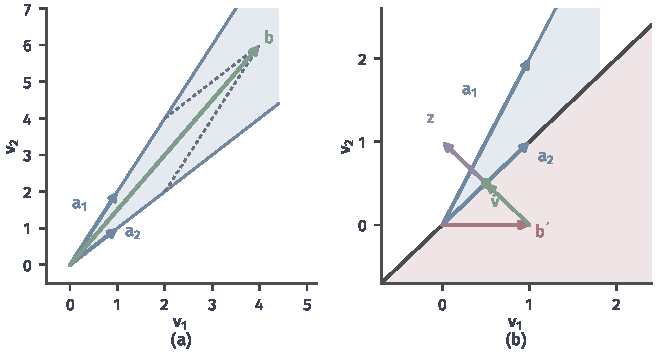
\includegraphics[width=112mm]{figures/05-optimization/01-linear-programming/matplotlib/lp-farkas-cone/figure.pdf}
 \caption{Farkas引理的几何。蓝色箭头是两列$\bm{a}_1,\bm{a}_2$，浅蓝区域是它们张成的锥。(a)~$\bm{b}=(4,6)^\top$在锥内，灰色虚线是$\bm{b}=2\bm{a}_1+2\bm{a}_2$的分解。(b)~$\bm{b}'=(1,0)^\top$在锥外，绿点$\widehat{\bm{v}}$是锥上最近的点，紫色箭头$\bm{z}=\widehat{\bm{v}}-\bm{b}'$是分离超平面（深灰线）的法向量；浅红半平面是$\bm{z}^\top\bm{v}<0$的一侧，$\bm{b}'$在其中，整个锥在另一侧。}
 \label{fig:lp-farkas-cone}
\end{BookInlineFigure}

\paragraph{强对偶}
现在回答开头的问题：只要原始问题可行且最优值有限，最好的下界就等于最优值，这个结论称为\term{强对偶}（strong duality）。

\begin{theorem}[线性规划强对偶]
 \label{thm:lp-strong-duality}
 若标准型~\eqref{eq:lp-standard}可行且最优值$p^\star$有限，则对偶问题~\eqref{eq:lp-dual}有最优解，并且
 \begin{equation}
  d^\star=p^\star.
  \label{eq:lp-strong-duality}
 \end{equation}
\end{theorem}

\begin{proof}
 只需找到$(\bm{y},\bm{s})$对偶可行，且$\bm{b}^\top\bm{y}\geq p^\star$，弱对偶就会迫使等号成立。把要求写成带非负变量的等式组，引入$r\geq0$，令$\bm{y}=\bm{y}^{+}-\bm{y}^{-}$：
 \[
  \bm{A}^\top\bm{y}^{+}-\bm{A}^\top\bm{y}^{-}+\bm{s}=\bm{c},\qquad
  \bm{b}^\top\bm{y}^{+}-\bm{b}^\top\bm{y}^{-}-r=p^\star.
 \]

 假设这个系统没有非负解。由Farkas引理，存在$\bm{z}\in\mathbb{R}^n$和$\sigma\in\mathbb{R}$，对系数矩阵的四组列分别满足
 \[
  \bm{A}\bm{z}+\sigma\bm{b}\geq\bm{0},\quad
  -\bm{A}\bm{z}-\sigma\bm{b}\geq\bm{0},\quad
  \bm{z}\geq\bm{0},\quad
  -\sigma\geq0,
 \]
 并且右端的内积为负，即$\bm{c}^\top\bm{z}+\sigma p^\star<0$。记$\tau=-\sigma\geq0$，前两式合起来得到
 \[
  \bm{A}\bm{z}=\tau\bm{b},\qquad\bm{z}\geq\bm{0},\qquad\bm{c}^\top\bm{z}<\tau p^\star.
 \]

 若$\tau>0$，则$\bm{z}/\tau$是原始可行点，目标值小于$p^\star$，矛盾。若$\tau=0$，则$\bm{A}\bm{z}=\bm{0}$，$\bm{z}\geq\bm{0}$，$\bm{c}^\top\bm{z}<0$。任取可行点$\widehat{\bm{x}}$，$\widehat{\bm{x}}+t\bm{z}$对一切$t\geq0$可行，目标趋于$-\infty$，与$p^\star$有限矛盾。

 所以系统有解，得到对偶可行的$(\bm{y},\bm{s})$和$\bm{b}^\top\bm{y}=p^\star+r\geq p^\star$。由弱对偶，$\bm{b}^\top\bm{y}\leq p^\star$，因此$\bm{b}^\top\bm{y}=p^\star$，这个$(\bm{y},\bm{s})$是对偶最优解。
\end{proof}

证明里两种情形各用了一个条件：$\tau>0$时用到$p^\star$是下确界，$\tau=0$时用到问题可行且有下界。线性规划的强对偶不需要其他条件。一般的凸问题则不然，第~\ref{chap:duality}章会在Lagrange函数的框架下说明，零间隙还需要额外的假设。

\paragraph{互补松弛与零间隙证书}
强对偶告诉我们证书一定存在，弱对偶告诉我们怎样核对它。把两者合起来，就是线性规划的最优性判别。

\begin{theorem}[零间隙证书与互补松弛]
 \label{thm:lp-optimality-certificate}
 设标准型的$\bm{x}$和$(\bm{y},\bm{s})$满足
 \begin{equation}
  \bm{A}\bm{x}=\bm{b},\quad\bm{x}\geq\bm{0},\qquad
  \bm{A}^\top\bm{y}+\bm{s}=\bm{c},\quad\bm{s}\geq\bm{0}.
  \label{eq:lp-pd-feasible}
 \end{equation}
 则下面三条等价：$\bm{x}$和$(\bm{y},\bm{s})$分别是原始、对偶最优解；$\bm{c}^\top\bm{x}=\bm{b}^\top\bm{y}$；对每个$j$，
 \begin{equation}
  x_js_j=0.
  \label{eq:lp-complementary}
 \end{equation}
\end{theorem}

\begin{proof}
 由式~\eqref{eq:lp-weak-duality}，第二条等价于$\bm{x}^\top\bm{s}=0$。$\bm{x}^\top\bm{s}$是非负数$x_js_j$之和，为零当且仅当每一项为零，这就是第三条。第二条推出第一条是弱对偶的结论。反过来若两者都最优，由强对偶知两个最优值相等，得到第二条。
\end{proof}

式~\eqref{eq:lp-complementary}称为\term{互补松弛}（complementary slackness）。它说的是，每对$(x_j,s_j)$中至少有一个为零。用价格的语言：正在生产的产品没有多余的利润，有多余的资源价格为零。第~\ref{chap:lp-interior-point}章的算法正是围绕这组方程组织的。

有了最优解的猜测，互补松弛还能反过来求出价格。车间问题中$\bm{x}^\star=(2,2,0,0)^\top$，$x_1,x_2>0$要求$s_1=s_2=0$，也就是
\[
 y_1+2y_2=-3,\qquad y_1+y_2=-2.
\]
解得$\bm{y}=(-1,-1)^\top$，再算出其余的对偶松弛：
\[
 s_3=-y_1=1,\qquad s_4=-y_2=1.
\]
$\bm{s}=(0,0,1,1)^\top\geq\bm{0}$，对偶可行，并且$\bm{b}^\top\bm{y}=-10=\bm{c}^\top\bm{x}^\star$。这一对点就是最优性的完整证书。

不是最优的顶点通不过同样的检查。取$(3,0)$，即$\bm{x}=(3,0,1,0)^\top$。$x_1,x_3>0$要求$s_1=s_3=0$，于是
\[
 y_1=0,\qquad y_2=-\frac32,\qquad s_2=-2-y_1-y_2=-\frac12<0.
\]
满足互补松弛的$\bm{y}$只有这一个，它不对偶可行，所以$(3,0)$不是最优解。

这个判别有直接的几何含义。回到平面上，顶点处的活动约束有各自的外法向量。互补松弛说的是，利润向量$\bm{p}$是活动约束法向量的非负组合。图~\ref{fig:lp-normal-cone}在两个顶点上比较：$(2,2)$处$\bm{p}=1\cdot\bm{n}_1+1\cdot\bm{n}_2$，系数正是价格$\bm{u}=(1,1)$；$(3,0)$处活动约束的法向量是$\bm{n}_2=(2,1)$和$\bm{n}_3=(0,-1)$，分解
\[
 \begin{bmatrix}3\\2\end{bmatrix}=\frac32\begin{bmatrix}2\\1\end{bmatrix}-\frac12\begin{bmatrix}0\\-1\end{bmatrix}
\]
含负系数，$\bm{p}$在锥外，负系数$-1/2$正是上面算出的$s_2$。

\begin{BookInlineFigure}
 \centering
 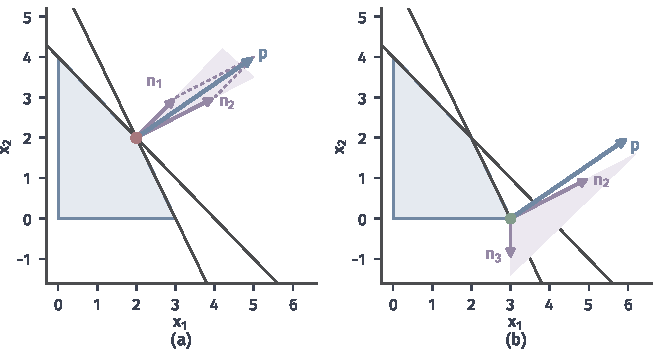
\includegraphics[width=112mm]{figures/05-optimization/01-linear-programming/matplotlib/lp-normal-cone/figure.pdf}
 \caption{互补松弛的几何。紫色箭头是顶点处活动约束的外法向量，浅紫区域是它们张成的锥，蓝色箭头是利润向量$\mathbf{p}=(3,2)$。(a)~$(2,2)$处，$\mathbf{p}$在锥内，是两个法向量的正组合（紫色虚线），该顶点最优。(b)~$(3,0)$处，$\mathbf{p}$在锥外，该顶点不是最优解。}
 \label{fig:lp-normal-cone}
\end{BookInlineFigure}

价格还有边际价值的含义。把工时从$4$增加到$5$，新的最优产量是$(1,4)$，利润$11$，恰好增加$u_1=1$。这种关系只在一定范围内成立，第~\ref{chap:simplex-method}章固定最优基时会算出这个范围。

\paragraph{三种结局的证书}
线性规划只有三种结局，每种都有可以独立核对的证据。有最优解时，证书是满足式~\eqref{eq:lp-pd-feasible}和式~\eqref{eq:lp-complementary}的一对点。不可行时，证书是满足式~\eqref{eq:lp-farkas-dual}的$\bm{z}$。无下界时，证书是一个可行点加上满足下式的方向：
\begin{equation}
 \bm{A}\bm{d}=\bm{0},\qquad\bm{d}\geq\bm{0},\qquad\bm{c}^\top\bm{d}<0.
 \label{eq:lp-unbounded-certificate}
\end{equation}

两个问题的结局也互相牵制。原始无下界时，对偶不可能有可行点，否则弱对偶会给出有限下界，所以对偶不可行。由对称性，对偶无上界时原始不可行。两者都不可行的情形确实存在，例如
\[
 \min\ -x_1-x_2\quad\text{s.t.}\quad x_1-x_2=1,\quad-x_1+x_2=1,\quad\bm{x}\geq\bm{0}.
\]
两个等式相加得到$0=2$，原始不可行；对偶约束$y_1-y_2\leq-1$和$-y_1+y_2\leq-1$相加得到$0\leq-2$，对偶也不可行。

这个例子中方向$\bm{d}=(1,1)^\top$满足式~\eqref{eq:lp-unbounded-certificate}，但没有可行的起点，它什么也说明不了。所以报告无下界时，可行点和方向缺一不可。表~\ref{tab:lp-outcomes}列出全部可能的组合。

\begin{BookInlineTable}
 \centering
 \begin{tabular}{llll}
  \toprule
  原始＼对偶 & 有最优解 & 无上界 & 不可行 \\
  \midrule
  有最优解 & 可能，且$p^\star=d^\star$ & 不可能 & 不可能 \\
  无下界 & 不可能 & 不可能 & 可能 \\
  不可行 & 不可能 & 可能 & 可能 \\
  \bottomrule
 \end{tabular}
 \caption{原始问题与对偶问题结局的组合。两个“有最优解”以外的“不可能”分别由强对偶、弱对偶和对称性得到。}
 \label{tab:lp-outcomes}
\end{BookInlineTable}

\paragraph{图中的流问题}
第~\ref{sec:lp-formulation}节的网络流实例能让对偶问题有具体的含义。关联矩阵~\eqref{eq:lp-network-data}的列是$\bm{a}_{i,j}=\bm{e}_i-\bm{e}_j$，所以$\bm{a}_{i,j}^\top\bm{y}=y_i-y_j$，对偶约束是逐弧的不等式，这里$\bm{e}_i$是第$i$个单位向量：
\begin{equation}
 s_{i,j}=c_{i,j}-(y_i-y_j)\geq0.
 \label{eq:lp-network-dual}
\end{equation}
$y_i$是节点上的数，可以读成“从节点$i$把一单位货物送到终点的费用估计”，这种量通常称为节点势。式~\eqref{eq:lp-network-dual}要求沿弧走一步，费用估计的下降不能超过这条弧的费用。对偶目标$\bm{b}^\top\bm{y}=y_1-y_4$是起点和终点的势差。

矩阵的四行线性相关，这时$\bm{y}$可以整体加一个常数而不影响任何$y_i-y_j$，所以取$y_4=0$，这相当于删去第四行。令最短路$1\to2\to3\to4$上的三条弧都取等号，得到
\[
 y_3=2,\qquad y_2=y_3+1=3,\qquad y_1=y_2+2=5.
\]
其余两条弧的对偶松弛为
\[
 s_{1,3}=5-(5-2)=2,\qquad s_{2,4}=6-(3-0)=3.
\]

路径$1\to2\to3\to4$的流量为$1$，总费用$2+1+2=5$，而$\bm{b}^\top\bm{y}=5-0=5$，两者相等。图~\ref{fig:lp-network-dual}显示了这份证书，互补松弛说的是：只有$s_{i,j}=0$的弧上才允许有流量。

\begin{BookInlineFigure}
 \centering
 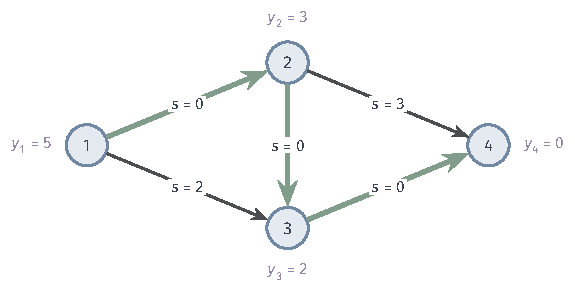
\includegraphics[width=97mm]{figures/05-optimization/01-linear-programming/tikz/lp-network-dual/figure.pdf}
 \caption{图~\ref{fig:lp-network-instance}实例的对偶证书。节点旁的紫色数字是节点势$y_i$，弧旁是对偶松弛$s_{i,j}$。绿色粗线是流量为$1$的最短路，这些弧上$s_{i,j}=0$，其余两条弧无流量。}
 \label{fig:lp-network-dual}
\end{BookInlineFigure}

这份证书正是图算法中逐弧检查的最优性条件。最短路的逐弧不等式和最小费用流的节点势都是对偶可行性，可参考\BookChapterRef{chap:shortest-paths}{卷三第3章“最短路”}；最大流最小割定理也是这种配对关系的特例，割给出流量的上界，可参考\BookChapterRef{chap:max-flow-min-cut}{卷三第5章“最大流与最小割”}。一般凸问题的对偶由第~\ref{chap:duality}章用Lagrange函数统一处理，线性规划是其中条件最宽松的情形。

\section{线性松弛}
\label{sec:lp-relaxation}

产品如果只能整批生产，变量就必须取整数。于是要问：去掉整数要求之后，连续问题的解和最优值能告诉我们整数问题的什么？回答分三层：最优值总能给出一个界；在特殊的矩阵结构下，顶点自动是整数；一般情形下，连续解还要经过专门论证的处理，才能变成原问题的可行解。

\paragraph{整数问题与它的松弛}
在标准型或不等式形式的线性规划上再要求变量取整数，就得到\term{整数线性规划}（integer linear programming）。设
\begin{equation}
 p_{\mathrm{I}}=\min\{\bm{c}^\top\bm{x}:\bm{x}\in\bm{C},\ \bm{x}\in\mathbb{Z}^n\},
 \qquad
 p_{\mathrm{R}}=\min\{\bm{c}^\top\bm{x}:\bm{x}\in\bm{C}\}.
 \label{eq:lp-relaxation-values}
\end{equation}
去掉整数要求后的问题称为原问题的\term{线性松弛}（linear relaxation）。这里的$\bm{C}$可以是任何多面体。

松弛扩大了可行集，最小化时最优值只会变小或不变。这是下面定理的全部内容，也是松弛提供的最基本的信息。

\begin{theorem}[松弛给出下界]
 \label{thm:lp-relaxation-bound}
 若整数问题可行且松弛的最优值有限，则
 \begin{equation}
  p_{\mathrm{R}}\leq p_{\mathrm{I}}.
  \label{eq:lp-relaxation-bound}
 \end{equation}
 若松弛有一个最优解是整数向量，则它也是整数问题的最优解，且等号成立。
\end{theorem}

\begin{proof}
 整数问题的可行点都在$\bm{C}$中，在较大的集合上取最小值不会更大，得到式~\eqref{eq:lp-relaxation-bound}。若松弛的最优解$\bm{x}$是整数向量，它对整数问题可行，于是
 \[
  p_{\mathrm{I}}\leq\bm{c}^\top\bm{x}=p_{\mathrm{R}}.
 \]
 再与式~\eqref{eq:lp-relaxation-bound}合并，等号成立。
\end{proof}

用一个具体的整数问题走一遍。把车间的原料增加到$7$份，利润系数改成$(3,1)$，并要求产量取整数：
\[
 \max\ 3x_1+x_2\quad\text{s.t.}\quad x_1+x_2\leq4,\quad2x_1+x_2\leq7,\quad\bm{x}\geq\bm{0},\quad\bm{x}\in\mathbb{Z}^2.
\]
松弛的四个顶点是$(0,0),(7/2,0),(3,1),(0,4)$，对应的利润依次是
\[
 0,\qquad\frac{21}{2},\qquad10,\qquad4.
\]
所以松弛的最优解是$(7/2,0)$，最优利润$21/2$。按$x_1$的取值逐个比较可行的整数点，$x_1$固定时$x_2$取最大，四种情形的利润依次是
\[
 x_1=0:\ 4,\qquad x_1=1:\ 6,\qquad x_1=2:\ 8,\qquad x_1=3:\ 10.
\]
$x_1\geq4$时原料不够，所以整数问题的最优解是$(3,1)$，利润$10$。这里是最大化，松弛给出的是上界，写成最小化$-3x_1-x_2$时，就是$p_{\mathrm{R}}=-21/2\leq-10=p_{\mathrm{I}}$。

\paragraph{舍入不是免费的}
最直接的想法是把松弛解舍入成整数。图~\ref{fig:lp-rounding}显示这个想法的问题。$(7/2,0)$向上取整得到$(4,0)$，用掉$8$份原料，不可行。向下取整得到$(3,0)$，可行，利润只有$9$，也不是最优。真正的最优解$(3,1)$在$x_2$上离松弛解差了一整个单位，它不是任何一种舍入的结果。

\begin{BookInlineFigure}
 \centering
 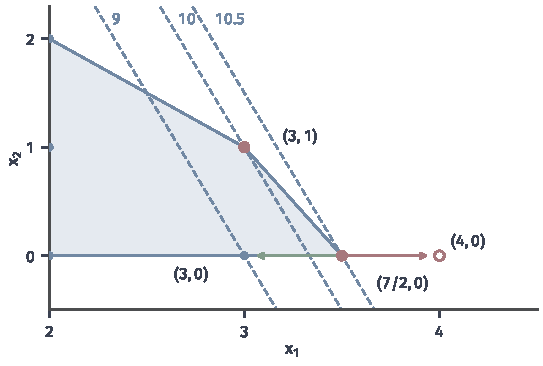
\includegraphics[width=92mm]{figures/05-optimization/01-linear-programming/matplotlib/lp-rounding/figure.pdf}
 \caption{舍入松弛解。蓝点是可行的整数点，蓝色虚线是利润$9$、$10$、$10.5$的等值线。松弛最优解$(7/2,0)$（红点，位于右下顶点）向右舍入到不可行的$(4,0)$（红色空心点），向左舍入到利润只有$9$的$(3,0)$；整数最优解是红点$(3,1)$。}
 \label{fig:lp-rounding}
\end{BookInlineFigure}

松弛最优值虽然不直接给出解，却给出了一个证明的工具。目标系数和变量都是整数时，$p_{\mathrm{I}}$也是整数，所以下界可以向上取整：
\[
 p_{\mathrm{I}}\geq\lceil p_{\mathrm{R}}\rceil=\Bigl\lceil-\frac{21}{2}\Bigr\rceil=-10.
\]
而$(3,1)$的目标值恰好是$-10$，这就证明了它是最优的，不需要枚举。一般情形下，松弛最优值和某个可行整数点的目标值夹出的区间，是对整数最优值的一个估计，这个区间的宽度取决于松弛有多紧。

$p_{\mathrm{I}}-p_{\mathrm{R}}$称为这个实例的\term{整数间隙}（integrality gap），这里是$1/2$。整数间隙衡量松弛对原问题的逼近程度，与求解松弛的算法无关。

\paragraph{整数顶点：全幺模}
既然线性规划的最优解可以在顶点取得，顶点若都是整数，整数约束就没有额外的代价。对比图~\ref{fig:lp-integer-hull}的两个多面体，它们的矩阵相同，右端不同：原料为$6$时四个顶点都是整数，原料为$7$时出现了分数顶点$(7/2,0)$。顶点是否整数，到底由什么决定？

\begin{BookInlineFigure}
 \centering
 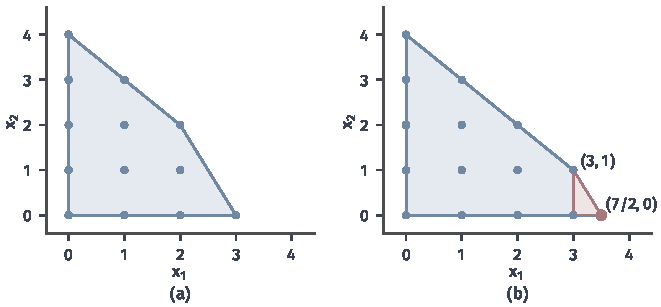
\includegraphics[width=112mm]{figures/05-optimization/01-linear-programming/matplotlib/lp-integer-hull/figure.pdf}
 \caption{相同的约束矩阵，不同的右端。蓝点是可行的整数点。(a)~原料为$6$，四个顶点都是整数。(b)~原料为$7$，右下顶点$(7/2,0)$是分数，红色小三角形是松弛比全体整数点的凸包多出的部分。}
 \label{fig:lp-integer-hull}
\end{BookInlineFigure}

答案在定义基本解的式~\eqref{eq:lp-basic-solution}里。由Cramer法则，
\[
 (\bm{x}_B)_i=\frac{\det\bm{A}_B^{(i)}}{\det\bm{A}_B},
\]
其中$\bm{A}_B^{(i)}$是把$\bm{A}_B$的第$i$列换成$\bm{b}$得到的矩阵。$\bm{A}$和$\bm{b}$都是整数时分子是整数，分数只能来自分母。如果基矩阵的行列式总是$\pm1$，顶点就一定是整数。图~\ref{fig:lp-integer-hull}(b)的分数顶点来自基$\{1,3\}$，它的行列式是$-2$，分母是$2$，而$7$是奇数；$b_2=6$时$6/2$仍是整数，分母恰好被消去。

\begin{definition}[全幺模矩阵]
 \label{def:lp-tu}
 若矩阵$\bm{A}$的每个方子矩阵的行列式都属于$\{0,1,-1\}$，就称$\bm{A}$是\term{全幺模矩阵}（totally unimodular matrix）。
\end{definition}

特别地，全幺模矩阵的元素都只能是$0,\pm1$。这个条件对所有方子矩阵提出要求，而不只是对基矩阵，这样它才能在加松弛变量、删冗余行这些改写后保持下来。

\begin{theorem}[全幺模与整数顶点]
 \label{thm:lp-tu-integral}
 设$\bm{A}$满行秩且全幺模，$\bm{b}$是整数向量。则$\bm{C}$的每个基本可行解都是整数向量。若问题可行且最优值有限，则存在整数最优解，从而
 \begin{equation}
  p_{\mathrm{I}}=p_{\mathrm{R}}.
  \label{eq:lp-tu-exact}
 \end{equation}
\end{theorem}

\begin{proof}
 任取基$B$。$\bm{A}_B$是可逆的方子矩阵，所以$\det\bm{A}_B=\pm1$。由Cramer法则，$\bm{x}_B$的每个分量都是整数行列式除以$\pm1$，是整数。第二句由定理~\ref{thm:lp-optimal-bfs}和定理~\ref{thm:lp-relaxation-bound}得到。
\end{proof}

不等式形式也可以用。若$\bm{A}$全幺模，则$[\bm{A}\ \ \bm{I}]$也全幺模：它的方子矩阵若含单位矩阵的列，这一列至多有一个非零元，按这一列展开，行列式化成$\bm{A}$的更小子矩阵的行列式，或者为零。于是不等式约束$\bm{A}\bm{x}\leq\bm{b}$，$\bm{x}\geq\bm{0}$在加了松弛变量之后满足定理的条件，变量的整数上界也可以同样处理。

定理的每个条件都起作用。$\bm{A}$全幺模但$\bm{b}$不是整数时，顶点就不是整数，例如$x_1\leq1/2$，$x_1\geq0$的顶点$1/2$。反过来，全幺模只是充分条件：车间矩阵含元素$2$，不是全幺模的，但$b_2=6$时顶点恰好都是整数。

定理说的是基本可行解，不是所有最优解。图~\ref{fig:lp-optimal-face}(b)那样有整条最优边的情形，边上的点可以不是整数，所以要得到整数解，必须取到顶点。

\paragraph{网络矩阵是全幺模的}
最重要的全幺模矩阵来自有向图。这正是图上的最短路、最大流、最小费用流可以用连续方法求整数解的原因。

\begin{theorem}[关联矩阵全幺模]
 \label{thm:lp-incidence-tu}
 设矩阵的每一列至多有一个$+1$、至多有一个$-1$，其余元素为零。有向图的关联矩阵就是这样的矩阵。这样的矩阵是全幺模的。
\end{theorem}

\begin{proof}
 对方子矩阵$\bm{D}$的阶数$k$归纳。$k=1$时元素属于$\{0,\pm1\}$。设$k>1$，$\bm{D}$的列也满足“至多一个$+1$、至多一个$-1$”，分三种情形。

 若某列全为零，$\det\bm{D}=0$。若某列恰有一个非零元，按这一列展开，$\det\bm{D}$等于$\pm$一个$k-1$阶子矩阵的行列式，由归纳假设属于$\{0,\pm1\}$。若每一列都恰有一个$+1$和一个$-1$，则所有行相加是零向量，$\det\bm{D}=0$。
\end{proof}

网络矩阵~\eqref{eq:lp-network-data}不是满行秩的，删去一行之后仍是全幺模矩阵的子矩阵，定理~\ref{thm:lp-tu-integral}可以使用。所以整数供需量、整数容量的最小费用流问题，线性规划的顶点解就是整数流，这正是第~\ref{sec:lp-duality}节实例中的最短路自动取$0$或$1$的原因。

二部图的情形也可以化成这个定理。把无向边看成两个非零元都是$+1$的列，二部图把顶点分成两侧，把一侧对应的行乘以$-1$，列就有了一个$+1$和一个$-1$，行列式只改变符号，所以二部图的关联矩阵也是全幺模的。这解释了指派问题的连续解为何能取整数，可参考\BookChapterRef{chap:bipartite-matching-assignment}{卷三第6章“二部图匹配与指派”}。

\paragraph{整数点的凸包}
全幺模解决了一类问题，一般情形还可以这样理解。有限个点$\bm{v}_1,\ldots,\bm{v}_k$的凸包是它们全部的加权平均，权重非负且和为$1$。线性目标在凸包上的最小值，等于在这些点上的最小值，因为加权平均不会比最小的项更小。

所以，若能把全体整数可行点的凸包用线性不等式写出来，整数问题就成了线性规划，图~\ref{fig:lp-integer-hull}(a)就是这种幸运的情形，松弛恰好等于这个凸包。图~\ref{fig:lp-integer-hull}(b)中松弛比凸包多了一块，多出来的部分造成了整数间隙。困难在于，一般的整数问题的凸包写不出来，不等式的条数可能随规模急剧增长。

\paragraph{一般情形：分数顶点}
图中只要出现奇圈，上面的论证就失效。考虑三个顶点的完全图（三角形），要选出尽量少的顶点，使每条边至少有一个端点被选中。这称为\term{顶点覆盖}（vertex cover）。用$x_i\in\{0,1\}$表示是否选中顶点$i$，问题是
\begin{equation}
 \min\ x_1+x_2+x_3
 \quad\text{s.t.}\quad x_1+x_2\geq1,\quad x_2+x_3\geq1,\quad x_1+x_3\geq1.
 \label{eq:lp-triangle-cover}
\end{equation}
松弛把$x_i\in\{0,1\}$放宽为$x_i\geq0$。三条约束取等号解出的点是
\[
 \bm{x}=\Bigl(\frac12,\frac12,\frac12\Bigr)^\top,\qquad\text{目标值}\ \frac32.
\]

它确实是松弛的最优解。把三条约束相加，得到$2(x_1+x_2+x_3)\geq3$，这正是取权重$(1/2,1/2,1/2)$的对偶证书，于是$p_{\mathrm{R}}=3/2$。

分数从哪里来？三条约束的系数矩阵是
\[
 \bm{E}=\begin{bmatrix}1&1&0\\0&1&1\\1&0&1\end{bmatrix},\qquad\det\bm{E}=2.
\]
行列式是$2$，所以不是全幺模矩阵，Cramer法则的分母正是$2$。三角形是奇圈，不能分成两侧，二部图的变号办法用不上。

整数问题的最优值是$2$：只选一个顶点时，对边的两端都没被选中，这条边没有被覆盖，所以至少选两个；选两个正好够。图~\ref{fig:lp-triangle-cover}对比了三种取值，这个实例的整数间隙是$2-3/2=1/2$。

\begin{BookInlineFigure}
 \centering
 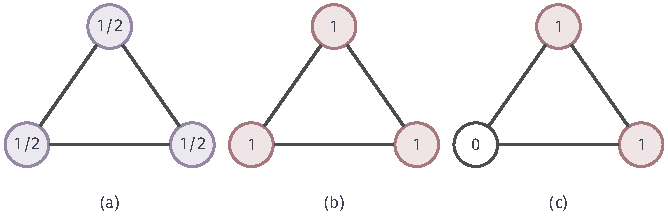
\includegraphics[width=112mm]{figures/05-optimization/01-linear-programming/tikz/lp-triangle-cover/figure.pdf}
 \caption{三角形上的顶点覆盖。圆内的数字是变量取值。(a)~松弛的最优解，三个变量都是$1/2$，目标值$3/2$。(b)~按阈值$1/2$舍入，三个变量都变成$1$，可行，目标值$3$。(c)~整数最优解之一，选两个顶点，目标值$2$。}
 \label{fig:lp-triangle-cover}
\end{BookInlineFigure}

\paragraph{从松弛解恢复可行解}
一般情形下，松弛解未必是整数，需要一个恢复步骤。恢复之后要分别回答两个问题：得到的点可行吗？目标值损失了多少？这两件事都要针对具体的约束结构来证明。前面的车间例子说明，随手舍入可能直接破坏可行性。

顶点覆盖是能够完整论证的例子。设无向图的顶点集为$V$，边集为$E$，顶点权重$w_i\geq0$。求解松弛
\[
 \min\ \sum_{i\in V}w_ix_i\quad\text{s.t.}\quad x_i+x_j\geq1\ \ (\{i,j\}\in E),\quad\bm{x}\geq\bm{0},
\]
得到最优解$\bm{x}^\star$，然后按阈值舍入：$x_i^\star\geq1/2$时取$\widehat{x}_i=1$，否则取$\widehat{x}_i=0$。

\begin{theorem}[顶点覆盖的阈值舍入]
 \label{thm:lp-cover-rounding}
 上述$\widehat{\bm{x}}$是可行的顶点覆盖，并且
 \begin{equation}
  \sum_{i\in V}w_i\widehat{x}_i\leq2\,p_{\mathrm{R}}\leq2\,p_{\mathrm{I}}.
  \label{eq:lp-cover-rounding}
 \end{equation}
\end{theorem}

\begin{proof}
 可行性：对每条边$\{i,j\}$，$x_i^\star+x_j^\star\geq1$，两个数中至少有一个不小于$1/2$，相应的$\widehat{x}$取$1$，这条边被覆盖。

 目标值：按舍入规则，每个$i$都满足$\widehat{x}_i\leq2x_i^\star$。权重非负，逐项相加，得到
 \[
  \sum_{i\in V}w_i\widehat{x}_i\leq2\sum_{i\in V}w_ix_i^\star=2p_{\mathrm{R}}.
 \]
 第二个不等号是定理~\ref{thm:lp-relaxation-bound}。
\end{proof}

三角形上这个界是$3\leq2\cdot\frac32$，等号成立，实际的最优值是$2$。系数$2$不能靠这种比较再改善。在$k$个顶点的完全图上，取单位权重，把全部边的约束相加，每个顶点出现$k-1$次，得到
\[
 (k-1)\sum_ix_i\geq\frac{k(k-1)}{2},\qquad\text{即}\qquad\sum_ix_i\geq\frac{k}{2}.
\]
全取$1/2$可以达到这个下界，松弛最优值是$k/2$。整数解至多有一个顶点不选，否则两个不选的顶点之间的边没被覆盖，所以整数最优值是$k-1$。两者之比随$k$增大趋于$2$。

这个定理的两个结论都依赖顶点覆盖的结构：可行性靠“两个数之和不小于$1$”，误差靠权重非负。换一种约束，例如前面车间的问题，同样的阈值可能得到不可行的点。所以，线性松弛本身只提供界和一个出发点，恢复原问题可行解的方法要逐类设计，并单独论证可行性和误差保证。

松弛的界不紧或者恢复的解不够好时，还可以继续加入有效的不等式来收紧松弛，或者把问题分成子问题分别求解。这类方法都要反复求解线性规划，第~\ref{chap:simplex-method}章将说明怎样在约束增加之后，利用已有的基接着求解。

\section{本章小结}
\label{sec:lp-summary}

回到章首的车间。等利润线在四边形上平移、最后停在角点，这幅图景在本章变成了三个可以计算的结论，它们的关系如图~\ref{fig:lp-summary-map}。

\begin{BookInlineFigure}
 \centering
 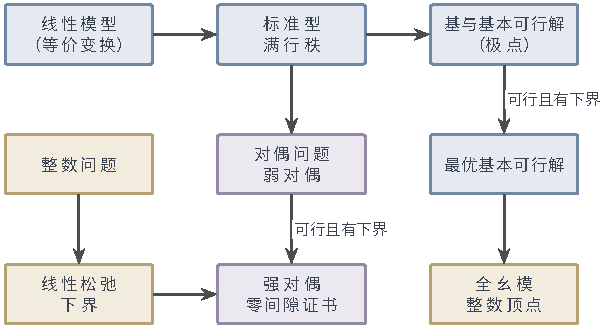
\includegraphics[width=102mm]{figures/05-optimization/01-linear-programming/tikz/lp-summary-map/figure.pdf}
 \caption{本章各部分的关系。蓝色框是原始问题的结构，紫色框是对偶与证书，黄色框是整数问题。箭头旁的文字是结论成立所需的条件。}
 \label{fig:lp-summary-map}
\end{BookInlineFigure}

第一，形式的统一。各种线性模型经过等价变换都能写成标准型，改写时松弛变量一一对应地保留可行集的形状，自由变量的分解保留最优值却可能多出角点。检查等式相容并删去冗余行之后，$\bm{A}$满行秩，基矩阵才有定义。

第二，解的位置。基本可行解就是可行集的极点，它由一个可逆的基矩阵解出；标准型只要可行且最优值有限，最优解就能在这有限个点中取得。非退化时换基对应沿边走到相邻顶点，退化时换基可能不移动，$\bm{u}\leq\bm{0}$时则得到无界可行方向。这个顶点结论依赖非负约束排除直线，含直线的多面体没有极点。

第三，解的证据。给约束配权重得到对偶问题，弱对偶说明对偶间隙等于$\bm{x}^\top\bm{s}$，因而非负，强对偶说明间隙可以精确为零。一对可行点满足互补松弛，就是最优性的完整证书，核对它只需矩阵乘法。表~\ref{tab:lp-summary}把这些结论和条件放在一起。

\begin{BookInlineTable}
 \centering
 \begin{tabular}{ll}
  \toprule
  结论 & 所需条件 \\
  \midrule
  基本可行解等于极点 & $\bm{A}$满行秩 \\
  存在最优基本可行解 & 标准型可行，最优值有限 \\
  沿边到不同的相邻顶点 & 基分量全为正，$\bm{u}$有正分量 \\
  弱对偶 & 两侧都可行 \\
  强对偶，对偶最优解存在 & 原始可行，最优值有限 \\
  松弛给出下界 & 最小化问题 \\
  顶点都是整数 & $\bm{A}$全幺模，$\bm{b}$是整数 \\
  \bottomrule
 \end{tabular}
 \caption{本章主要结论及其条件。}
 \label{tab:lp-summary}
\end{BookInlineTable}

整数问题是另一类问题。线性松弛提供一个界；全幺模配合整数右端保证顶点是整数，网络问题属于这一类；一般情形下松弛解可能是分数，恢复可行解需要针对具体结构论证可行性和误差。

本章说明了最优解在哪里、怎样核实，但没有给出高效的求解方法。第~\ref{chap:simplex-method}章沿着基本可行解换基前进，直到拿到零间隙证书。第~\ref{chap:lp-interior-point}章从可行集内部出发，保持$\bm{x}$和$\bm{s}$为正，逐步缩小互补松弛的残差。

